\chapter{Benchmarking Neuromorphic Vision}
\label{cha:bench}

%Today, increasing attention is being paid to research into spike-based neural computation both to gain a better understanding of the brain and to explore biologically-inspired computation.
%Within this field, the primate visual pathway and its hierarchical organisation have been extensively studied.
%Spiking Neural Networks (SNNs), inspired by the understanding of observed biological structure and function, have been successfully applied to visual recognition and classification tasks.
%In addition, implementations on neuromorphic hardware have enabled large-scale networks to run in (or even faster than) real time, making spike-based neural vision processing accessible on mobile robots.
%Neuromorphic sensors such as silicon retinas are able to feed such mobile systems with real-time visual stimuli.

The last two chapters have answered the main research question of this thesis showing that Spiking Neural Networks (SNNs) can be trained both on-line and off-line to achieve the equivalent cognitive capabilities of Artificial Neural Networks~(ANNs).
To provide meaningful comparisons between theses proposed SNN models and other existing methods within this rapidly advancing field of Neuromorphic Engineering~(NE), we propose that a large dataset of spike-based visual stimuli is needed and a corresponding evaluation methodology is also required to estimate the overall performance of SNN models and their hardware implementations.

%A new set of vision benchmarks for spike-based neural processing are now needed to measure progress quantitatively within this rapidly advancing field.
%
\section{Introduction}
\label{sec:chapt6_intro}
Today, increasing attention is being paid to research into spike-based neural computation both to gain a better understanding of the brain and to explore biologically-inspired computation.
Within this field, the primate visual pathway and its hierarchical organisation have been extensively studied.
SNNs have been successfully applied to visual recognition and classification tasks.
In addition, Neuromorphic hardware have enabled large-scale SNNs to run in (or even faster than) real time, and also made spike-based neural vision processing accessible on mobile robots.
Besides, neuromorphic sensors such as silicon retinas are able to feed such mobile systems with real-time visual stimuli.

A new set of vision benchmarks for spike-based neural processing are now needed to measure progress quantitatively within this rapidly advancing field.
%We propose that a large dataset of spike-based visual stimuli is needed to provide meaningful comparisons between different systems, and a corresponding evaluation methodology is also required to measure the performance of SNN models and their hardware implementations.
%
In this chapter we first propose an initial NE dataset based on standard computer vision benchmarks and that uses digits from the MNIST database.
This dataset is compatible with the state of current research on spike-based image recognition.
The corresponding spike trains are produced using a range of techniques: rate-based Poisson spike generation, rank order encoding, and recorded output from a silicon retina with both flashing and oscillating input stimuli.
In addition, a complementary evaluation methodology is presented to assess both model-level and hardware-level performance.
Finally, we demonstrate the use of the dataset and the evaluation methodology using an SNN model to validate the performance of the models and their hardware implementations.

With this dataset we hope to (1) promote meaningful comparisons between algorithms and neuromorphic platforms in the field of NE, (2) allow comparison with conventional non-spiking methods on image recognition, (3) provide an assessment of the state of the art in spike-based visual recognition, and (4) help researchers identify future directions and advance the field.

In Section~\ref{sec:chapt6_intro}, diverse neuromorphic vision tasks are introduced to illustrate the requirements for a unified spike-based dataset.
The rest of this chapter is structured as follows: Section~\ref{sec:method} elaborates the purpose and protocols of the proposed dataset and describes the sub-datasets and the methods employed to generate them; Section~\ref{sec:eval} demonstrates the suggested evaluation methodology for use with the dataset.
%The sub-datasets and their generation methods are described in detail in Section~\ref{sec:data}.
%In accordance with the dataset, its evaluation methodology is demonstrated in Section~\ref{sec:eval}.
Section~\ref{sec:test} presents an SNN case study as demonstrations of using the dataset to assess model performance and benchmark hardware platforms.
Finally, Section~\ref{sec:summ} summarises the chapter.


\section{Related Work}
\label{sec:chapt6_relate}
Researchers are using the capabilities created by rapid developments in neuromorphic engineering to address the dual aims of understanding brain functions and building brain-like machines~\citep{furber2007neural}.
Neuromorphic engineering has delivered biologically-inspired sensors such as DVS~(Dynamic Vision Sensor) silicon retinas~\citep{serrano2013128, delbruck2008frame, yang2015dynamic, posch2014retinomorphic}, which offer the prospect of low-cost visual processing thanks to their event-driven and redundancy-reducing style of information representation.
Moreover, SNN simulation tools~\citep{davison2008pynn, gewaltig2007nest, goodman2008brian} and neuromorphic hardware platforms~\citep{furber2014spinnaker,  schemmel2010wafer,benjamin2014neurogrid,merolla2014million} have been developed to allow exploration of the brain by mimicking its functions and developing large-scale practical applications~\citep{eliasmith2012large}.
%TODO Vision Recognition on SNNs. Aims: brain like -> feed_forward structure, accuracy, latency and energy efficiency.
Achieving the brain's energy efficiency motivates the development of neuromorphic hardware, since the human brain has a power consumption of only about 20~W~\citep{drubach2000brain}.
In the case of visual processing, the brain can accurately recognise objects remarkably quickly, e.g. in 200~ms in monkeys~\citep{fabre1998rapid}, even with short presentations (less than 100~ms) of the target objects~\citep{keysers2001speed}.
Such rapid and highly accurate recognition is the target of modelling spike-based visual recognition.


%In the case of visual processing, the central visual system consists of several cortical areas which, according to anatomical experiments, are placed in a hierarchical structure ~\citep{felleman1991distributed}.
%Fast object recognition takes place in the feed-forward hierarchy of one of the two central visual pathways, the ventral pathway, which mainly handles the `What' tasks.
%Biological studies have revealed that the information is unfolded along the ventral stream to the IT (Inferior Temporal) cortex~\citep{dicarlo2012does}.
%Inspired by these results, SNN models have successfully been adapted to computer vision tasks.  

%Bioligical inspiration
Inspired by biological studies of the visual ventral pathway, SNN models have successfully been adapted to visual recognition. \citet{riesenhuber1999hierarchical} proposed a quantitative modelling framework for object recognition with position-, scale- and view-invariance.
Their cortex-like model has been analysed on several datasets~\citep{serre2007robust}.
Recently~\citet{fu2012spiking} reported that their SNN implementation was capable of recognising facial expressions with a classification accuracy (CA) of 97.35\% on the JAFFE dataset~\citep{lyons1998coding} which contains 213 images of 7 facial expressions posed by 10 individuals.
%They employed simple integrate-and-fire~(IF) neurons with rank order coding (ROC) where the earliest pre-synaptic spikes have the strongest impact on the post-synaptic potentials.
According to~\citet{vanrullen2002surfing}, the first wave of spikes carry explicit information through the ventral stream and in each stage meaningful information is extracted and spikes are regenerated. 
Therefore, using one spike per neuron, similar to the first spiking wave in biology,~\citet{delorme2001face} reported 100\% and 97.5\% accuracies on the face identification task over
%changing  contrast and luminance 
training (40 individuals $\times$ 8 images) and testing data (40 individuals $\times$ 2 images).
%TODO move the two examples to algorithms part.
%In terms of vision recognition on neuromorphic hardware, TrueNorth~\citep{merolla2014million} has been used to detect and recognise five classes of object in the video clips of the Neovision2 Tower dataset.
%\citep{Qiao2015re} presented an analogue on-line learning neuromorphic classification system which responds selectively to images of cars and motorbikes selected from the Caltech 101 dataset.
%Generic training algorithms for pattern recognition~\citep{schmuker2014neuromorphic} and regression/classification tasks~\citep{thakur2016low} have been implemented on neuromorphic platforms.
%The Convolutional Neural Network (CNN), also known as the \textit{ConvNet}, developed by, is a widely-used model based on a cortex-like framework.
%\citep{hubel1962receptive} first discovered the model of orientation selectivity (simple cells) and pooling mechanism (complex cells) in the primary cortex in cats, which lay the foundation of the Convolutional Neural Network (CNN)~\citep{lecun1998gradient}.

Convolutional Neural Networks (ConvNets), inspired by the receptive fields of the visual cortex, have been implemented on spiking neurons.
An early Spiking ConvNet model identified the faces of 35 persons with a CA of 98.3\% exploiting simple integrate and fire neurons~\citep{matsugu2002convolutional}.
Another Spiking ConvNet model~\citep{zhao2014feedforward} was trained and tested both with DVS raw data and Leaky Integrate-and-Fire (LIF) neurons.
It was capable of recognising three moving postures with a CA of about 99.48\% and classifying hand-written digits with 88.14\% accuracy on the MNIST-DVS dataset (see Section~\ref{sec:data}).
In a further step forward,~\citet{camunas2012event} implemented a convolution processor module in hardware which could be combined with a DVS for high-speed recognition tasks.
The inputs of the ConvNet were continuous spike events instead of static images or frame-based videos. 
The chip was capable of detecting the four suits in a 52-card deck which was browsed rapidly in only 410 ms.
Similarly, a real-time gesture recognition model~\citep{liu2014real} was implemented on a neuromorphic system with a DVS as a front-end and a SpiNNaker~\citep{furber2014spinnaker} machine as the back-end, where LIF neurons built up the ConvNet configured with biological parameters.
In this study's largest configuration, a network of 74,210 neurons and 15,216,512 synapses used 290 SpiNNaker cores in parallel and reached 93.0\% accuracy. 

Spike-Timing-Dependent Plasticity (STDP) as a learning mechanism based on biological observations has been applied to vision tasks.
As mentioned in Chapter~\ref{cha:intro}, these models typically comprise only two neural layers and exploit STDP and/or Winner-Take-All~(WTA) circuits on the synaptic connections.
\citet{bichler2012extraction} demonstrated an unsupervised STDP learning model to classify car trajectories captured with a DVS retina. 
A similar model trained with STDP using a winner-take-all~(WTA) circuit was tested on a Poissonian spike presentation of the MNIST dataset achieving a performance of 95.0\%~\citep{diehl2015unsupervised}.
%Theoretical analysis~\citep{nessler2013bayesian} showed that unsupervised STDP was able to approximate a stochastic version of Expectation Maximisation, a powerful learning algorithm in machine learning.
Another STDP trained model tested on computer simulation reached a 93.3\% CA on MNIST and had the potential to be implemented using memristors~\citep{bill2014compound}. 
Adding synaptic internal state enabled STDP to work on bistable synapses, and this method achieved the best performance of 96.5\% among similar network architectures. 

Deep Neural Networks (DNNs) have exceeded human-level performance on image classification tasks~\citep{he2015delving}, but mainstream DNN research is focussed on continuous rather than spiking neural networks.
The spiking deep network has great potential to combine remarkable performance with energy-efficient training and operation.
Early research into spiking deep networks focussed on converting off-line trained deep network into SNNs~\citep{o2013real}.
The network was initially implemented on an FPGA and achieved a CA of 92.0\%~\citep{neil2014minitaur}, while a later implementation on SpiNNaker scored 95.0\%~\citep{Stromatias2015scalable}.
Recent advances have contributed to better translation by using modified units in a ConvNet~\citep{cao2015spiking} and tuning the weights and thresholds~\citep{diehl2015fast}.
The latter paper claims a state-of-the-art performance (99.1\% on the MNIST dataset) compared to the original ConvNet.
The current trend towards training Spiking DNNs on line using biologically-plausible learning methods is also promising.
An event-driven Contrastive Divergence (CD) training algorithm for Restricted Boltzmann Machines (RBMs) was proposed for Deep Belief Networks (DBNs) using LIF neurons with STDP synapses and verified on MNIST with a CA of 91.9\%~\citep{neftci2013event}.
The work extended to use stochastic synapses, and the recognition performance increased to 95.8\%~\citep{neftci2016stochastic}.


Despite the promising research on SNN-based vision recognition, there is no commonly used database in the format of spike stimuli.
In the studies listed above, all of the vision data used are in one of the following formats:
(1) raw grey-scale images data;
(2) pixel-intensity-driven rate-based Poisson spike trains;
(3) unpublished spike-based videos recorded from DVS silicon retinas.
However, in the field of conventional non-spiking computer vision, there are a number of datasets playing important roles at different times and with various objectives~\citep{lecun1998gradient,deng2009imagenet,blank2005actions,liu2009recognizing}.
%The MNIST~\citep{lecun1998gradient} dataset is a subset of the NIST hand-written digits dataset; due to its straightforward target of classifying real-world images, the plain format of the binary data and simple patterns, MNIST has been one of the most popular datasets in computer vision for over 20 years.
%ImageNet~\citep{deng2009imagenet} was put forward to provide researchers with a large-scale image database that currently contains 14,197,122 images;
%this dataset is a well-recognised benchmark test for the deep learning community, and many attempts have been made to improve the performance of machine learning algorithms on this dataset, as was done, for example, by \citep{krizhevsky2012imagenet}.
%As a good example of a database catching up with state-of-the-art technologies, Microsoft COCO aims to solve three problems - objects categorisation, context understanding and spatial labelling - in scene understanding by providing large-scale datasets (300,000+ images).
%Similar examples can be found in video datasets.
%Two early benchmarks, the KTH ~\citep{schuldt2004recognizing} and Weizmann~\citep{blank2005actions} datasets, have been used extensively in the past decade. 
%These videos were produced with scripted behaviours in a controlled environment (`in the lab').
%The YouTube Action Dataset~\citep{liu2009recognizing} targets recognising realistic actions from videos `in the wild';
%here the main challenge is in the massive variations due to the moving camera, background clutter, viewing angles, variable illumination and so on.
In consequence, a new set of spike-based vision datasets is now needed to quantitatively measure progress within the rapidly advancing field of spike-based visual recognition and to provide resources to support fair competition between researchers.

Apart from using spikes instead of the frame-based data used in conventional computer vision, new concerns arise when evaluating neuromorphic vision, such as latency and energy consumption, in addition to recognition accuracy.
These concerns naturally derive from the goal of spike-based visual recognition: mimicking the fast recognition with low-energy processing in the brain. 
%TODO better word to describe: what are the metrics and why needed
Therefore a set of common metrics for performance evaluation in spike-based vision is required to assess SNN models and their hardware implementations.
%, including evaluating trade-offs between simulation time, accuracy and power consumption.
%Benchmarking neuromorphic hardware with various network models will reveal the advantages and disadvantages of different platforms.
%Running various SNN benchmarks demonstrates the capability of a hardware platform to support model-specific configurations such as network size, topology, neural and synaptic models, learning algorithms and so on.
In this chapter we propose a large dataset of spike-based visual stimuli and a complementary evaluation methodology.
Just as research in this field is an expanding and evolving activity, the dataset will be adapted and extended to fit new requirements presented by advances in the field.



%\section{Related Work}
%\label{sec:Related}
%In conventional computer vision, there are a few datasets playing important roles at different times and with various objectives.
%\subsection{MNIST}
%The MNIST~\citep{lecun1998gradient} dataset is a subset of the NIST hand written digits dataset.
%The training set contains 60,000 patterns collected from approximately 250 writers.
%The testing set is composed of 10,000 patterns written by disjoint individuals which were not listed in the training set.
%All the digits in the dataset are of similar scale centring in a 28$ \times $28 image.
%Due to its straightforward target of classifying real-world images, the plain format of binary data and the simple patterns, MNIST has been one of the most popular datasets in computer vision for over 20 years.
%
%Many methods have been verified on this dataset: K-means, SVM, ConvNets, etc.
%The descending recognition error rate makes it nearly a solved problem, however some modifications, such as position shifts, scaling and noise, bring new challenges.
%Certainly, a spiking version of the dataset will be an interesting artificial distortion and draw attention to new methods and algorithms on the challenge. 
%
%\subsection{ImageNet~\citep{deng2009imagenet}}
%Since the new era of the 4th generation ANN, the DNN, a flow of successful applications have been reported.
%Meanwhile, training the deeper network triggers a huge demand for sample data.
%The purpose of putting forward ImageNet was to provide researchers with a large-scale image database, which matches nicely with DNN data requirements.
%Currently there are 14,197,122 images and 21,841 synsets indexed in the dataset\footnote{http://www.image-net.org/}.
%Synsets are meaningful concepts described with a few words or phrases, and they are organised in a hierarchy as in WordNet.%~\citep{deng2009imagenet}.
%The final goal of ImageNet is to provide about 1000 images for each of the 80,000 synsets in WordNet.
%In other words, there will be tens of millions of images tidily structured, accurately labelled and human annotated.
%The dataset is a well-recognised benchmark test for the deep learning community, and many attempts have been made to improve the performance of machine learning algorithms on this dataset, for example~\citep{krizhevsky2012imagenet}.
%
%\subsection{Microsoft COCO~\citep{lin2014microsoft}}
%As a good example of a database catching up with state-of-the-art technologies, Microsoft COCO aims to solve three problems in scene understanding by providing large-scale datasets.
%First is to categorise objects in their non-iconic views, such as being small, ambiguous or partially occluded.
%Secondly, understanding the context (contextual reasoning) of multiple objects in an image is necessary.
%Lastly, spatial labelling of the objects is a core analysis in scene understanding.
%Up to date, the dataset contains 300,000+ images, 2 million instances and 5 captions per image.
%
%\subsection{Action Datasets}
%Similar examples could be found in video datasets.
%Two early benchmarks, the KTH ~\citep{schuldt2004recognizing} and Weizmann~\citep{blank2005actions} datasets, have been used extensively in the past decade. 
%These videos were produced with scripted behaviours in a controlled environment (`in the lab').
%They contain single atomic actions, which are simple and neat: walking, running, sitting, etc.
%
%Taking the advantages of continuous spiking trains instead of frames of videos, spiking versions of such action datasets will be provided in our future work.
%A DVS simulation may be needed to convert frames of images into spikes.
%
%The YouTube Action Dataset~\citep{liu2009recognizing} targets recognising realistic actions from videos `in the wild'.
%Thanks to the digital era, unconstrained videos are abundant on the Internet, e.g. YouTube.
%This YouTube Action dataset is composed of 1,168 videos in 11 categories.
%The main challenge relies on the massive variations due to the moving camera, background clutter, viewing angles, illuminations and so on.
%It also aims to detect complex action (non-atomic), e.g. long jump, which consists of several continuous atomic actions.


\section{NE Dataset}
\label{sec:method}
\subsection{Guiding Principles}
The NE database we propose here is a developing and evolving dataset consisting of various spike-based representations of images and videos.
The spikes are either generated from spike encoding methods which convert images or frames of videos into spike trains, or recorded from DVS silicon retinas.
The spike trains are in the format of Address-Event Representation~(AER)~\citep{mahowald1992vlsi} data, which are suitable for both event-driven computer simulations and neuromorphic systems.
AER was originally proposed as a time-multiplexed spike communication protocol where each time a neuron produces a spike an event is generated that codes the spiking neuron's address on a fast time-multiplexed digital bus.
The recorded AER data consists of a list of events, each one containing the time stamp of a spike and the address of the neuron which generated the spike.
With the NE dataset we hope:
\begin{itemize}
	\item \textit{to promote meaningful comparisons between algorithms and neuromorphic platforms in the field of NE.}
	The NE dataset provides a unified format of AER data to meet the demands of spike-based visual stimuli.
	It also encourages researchers to publish and contribute their data to build up the NE dataset.
	\item \textit{to allow comparison with conventional non-spiking methods on image recognition.}
	We expect the dataset to support this comparison using spiking versions of existing vision datasets.
	Thus, conversion methods are required to transform datasets of images and frame-based videos into spike stimuli.
	More biologically-accurate and better information preserving schemes are welcome.
	%	With the growing understanding of biological vision, new methodologies and algorithms that can convert these conventional datasets into spikes in more biologically-accurate ways are welcome.
	%	Other spike representation schemes may do a better job of preserving information from the original stimuli.
	
	\item \textit{to provide an assessment of the state of the art in spike-based visual recognition.}
	To reveal the accuracy, speed, and energy-efficient recognition of neuromorphic approaches, we need not only a spike-based dataset but also an appropriate evaluation methodology.
	The evaluation methodology will be constantly improving along with the evolution of the dataset.
	\item \textit{to help researchers identify future directions and advance the field.}
	The development of the dataset and its evaluation methodology will introduce new challenges for the neuromorphic engineering community.
	However, these must represent an appropriate degree of difficulty: a too-easily-solved problem turns into a tuning competition, while a problem that is too difficult will not yield meaningful assessment.
	So suitable problems should continuously be added to promote future research.  
\end{itemize}


\subsection{The Dataset: NE15-MNIST}
\label{sec:data}
%Experiment setup/ collection method/ properties of each class/ etc.
The first proposed dataset in the benchmarking system is NE15-MNIST (Neuromorphic Engineering 2015 on MNIST).
NE15-MNIST is the spiking version of an original non-spiking dataset which was downloaded from the MNIST Database of Handwritten Digits~\citep{lecun1998gradient}  website\footnote{\url{http://yann.lecun.com/exdb/mnist/}}.
Due to its straightforward target of classifying real-world images, the plain format of the binary data and simple patterns, MNIST has been one of the most popular datasets in computer vision for over 20 years.
MNIST is a popular task among the neuromorphic vision research community.
The converted MNIST dataset consists of four subsets which were generated for different purposes:
\begin{itemize}
	\item \textit{Poissonian},
	which encodes each pixel as a Poisson spike train and is intended for benchmarking existing rate-based SNN models.
	\item \textit{FoCal~(Filter Overlap Correction ALgorithm)},
	to promote the study of spatio-temporal algorithms applied to recognition tasks using small numbers of input spikes.
	\item \textit{DVS recorded flashing input},
	to encourage research into fast recognition methods to mimic the rapid and accurate `core recognition' in the primate ventral visual pathway~\citep{dicarlo2012does}.
	\item \textit{DVS recorded moving input},
	to trigger the study of algorithms targeting continuous input from real-world sensors for implementation, for example, on mobile neuromorphic robots.
\end{itemize}
The dataset is published in the GitHub: \url{https://github.com/NEvision/NE15}.
\subsection{Data Description}
Two file formats are supported in the dataset: the jAER format~\citep{delbruck2008frame} (.dat or .aedat), and binary files in NumPy~\citep{numpyPython} (.npy) format.
%The AER interface has been widely used in neuromorphic systems, especially for vision sensors.
%The spikes are encoded as time events with corresponding addresses to convey information.
The spikes in jAER format, whether recorded from a DVS retina or artificially generated, can be displayed by the jAER software.
Figure~\ref{fig:zero}(a) is a snapshot of the software displaying a .aedat file which was recorded from a DVS retina~\citep{serrano2013128}.
The resolution of the DVS recorded data is 128$\times$128.
The second spike-based format used is a list of spike source arrays in PyNN~\citep{davison2008pynn}, a description language for building spiking neuronal network models.
Python code is provided for converting from either file format to the other.
The duration of the artificially-generated data can be configured using the Python code provided, while the recorded data varies in duration: 1~s for the flashing input, and 3.2 to 3.4~s for the moving input.




\begin{figure}[bht!]
	\centering
	%	\subfloat[A snapshot of jAER playing the DVS recorded spikes.]{
	%		\label{Fig:jaer}
	%		\includegraphics[width=0.22\textwidth]{dvs-128}
	%	}
	%	\subfloat[A snapshot of jAER playing Poissonian spike trains.]{
	%		\label{Fig:poisson}
	%		\includegraphics[width=0.22\textwidth]{zero-28-2}
	%	}\\
	%	\subfloat[The raster plot of the Poissonian spike trains.]{
	%		\label{Fig:raster}
	%		\includegraphics[width=0.48\textwidth]{zero}
	%	}
	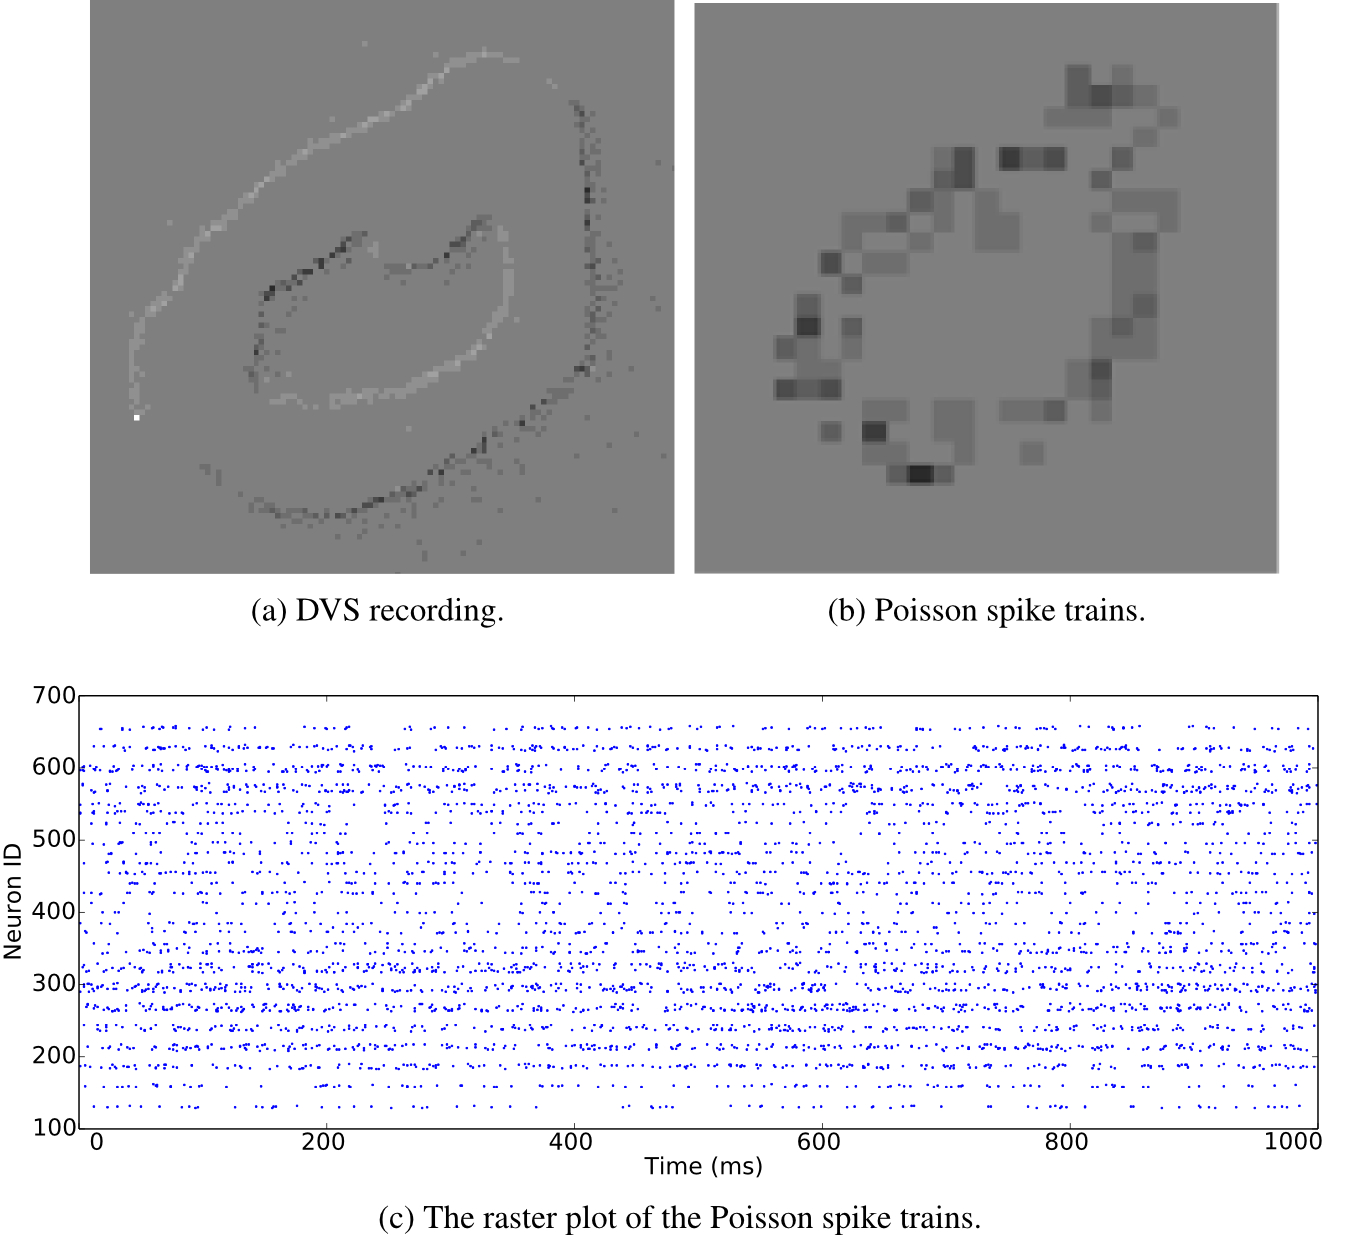
\includegraphics[width=0.8\textwidth]{pics_bench/fig1.jpg}
	\caption[Snapshots of the jAER software.]{
		Snapshots of the jAER software displaying spike-encoded videos.
		The same image of digit `0' is transformed into spikes by (a) DVS recording and (b) Poisson generation.
		(c) A raster plot of the Poisson spike trains.}
	\label{fig:zero}
\end{figure}

%\subsubsection{Data Description}	
\subsubsection{Poissonian}
\label{sec:poissonian}
The timing of spikes in the cortex is highly irregular~\citep{squire1998findings}.
%In the cortex, the timing of spikes is highly irregular~\citep{squire1998findings}.
An interpretation is that the inter-spike interval reflects a random process driven by the instantaneous firing rate.
If the generation of each spike is assumed to be independent of all other spikes, the spike train is seen as a Poisson process.
The spike rate can be estimated by averaging the pooled responses of the neurons.


As stated above, rate coding is generally used in presenting images as spike trains.
The spike rate of each neuron accords with the intensity of the corresponding pixel.
Instead of providing exact spike arrays, we share the Python code for generating the spikes.
Each recognition system may require different spike rates and durations.
The generated Poisson spike trains can be in both jAER and PyNN spike source array formats.
Thus, it is easy to visualise the digits and also to couple the spike trains into spiking neural networks.
Because different simulators generate random Poisson spike trains with different mechanisms, languages and codes, using the same dataset enables performance evaluation on different simulators without the confusion created by differences in input.
The same digit displayed in Figure~\ref{fig:zero}(a) can be converted into Poisson spike trains, see Figure~\ref{fig:zero}(b).
A raster plot of the Poisson spike trains is shown in Figure~\ref{fig:zero}(c).



\subsubsection{Rank Order Encoding}
A different way of encoding spikes is to use a rank order code; this means
keeping just the order in which the spikes fired and disregarding their exact timing.
Rank-ordered spike trains have been used in vision tasks under a biological plausibility constraint, making them a viable way of encoding images for neural applications~\citep{van2001rate,sen2009evaluating,masmoudi2010novel}.
%
%\begin{table}[tbh!]
%	\caption{Simulation parameters for FoCal ganglion cells}
%	\begin{center}
%		
%		
%		%		\bgroup
%		%		\def\arraych{0.1}
%		
%		\begin{tabular}{c c c c c c}
%			\begin{mycellS}{0.8cm}\centering Layer \end{mycellS}& 
%			\begin{mycellS}{1.1cm}\centering Centre type\end{mycellS}& 
%			\begin{mycellS}{1.1cm}\centering Matrix width \end{mycellS}&  
%			\begin{mycellS}{1.6cm}\centering Centre std. dev. ($\sigma_c$)\end{mycellS} & 
%			\begin{mycellS}{1.6cm}\centering Surround std. dev. ($\sigma_s$)\end{mycellS} & 
%			\begin{mycellS}{1.3cm}\centering Sampling resolution (cols,rows)\end{mycellS} \\
%			\hline
%			\begin{mycell}{0.8cm} 1  \end{mycell} &
%			\begin{mycell}{1.1cm} \textsc{OFF} \end{mycell}& 
%			\begin{mycell}{1.1cm} 3 \end{mycell}& 
%			\begin{mycell}{1.6cm}$0.8$ \end{mycell}& 
%			\begin{mycell}{1.6cm}$6.7 \times \sigma_c$ \end{mycell}&  
%			\begin{mycell}{1.6cm}1, 1 \end{mycell}\\
%			\begin{mycell}{0.8cm} 2 \end{mycell} & 
%			\begin{mycell}{1.1cm} \textsc{ON} \end{mycell} & 
%			\begin{mycell}{1.1cm} 11 \end{mycell}& 
%			\begin{mycell}{1.6cm}$1.04$ \end{mycell}& 
%			\begin{mycell}{1.6cm}$6.7 \times \sigma_c$ \end{mycell}& 
%			\begin{mycell}{1.6cm}1, 1 \end{mycell}\\
%			\begin{mycell}{0.8cm} 3 \end{mycell} &
%			\begin{mycell}{1.1cm} \textsc{OFF}\end{mycell} & 
%			\begin{mycell}{1.1cm} 61 \end{mycell}& 
%			\begin{mycell}{1.6cm}$8$ \end{mycell}& 
%			\begin{mycell}{1.6cm}$4.8 \times \sigma_c$ \end{mycell}& 
%			\begin{mycell}{1.6cm}5, 3\end{mycell} \\
%			\begin{mycell}{0.8cm} 4  \end{mycell} & 
%			\begin{mycell}{1.1cm} \textsc{ON} \end{mycell} & 
%			\begin{mycell}{1.1cm} 243 \end{mycell} &
%			\begin{mycell}{1.6cm}$10.4$\end{mycell} & 
%			\begin{mycell}{1.6cm}$4.8 \times \sigma_c$\end{mycell} & 
%			\begin{mycell}{1.6cm}5, 3 \end{mycell}
%		\end{tabular}
%		%		\egroup
%	\end{center}
%	\label{tab-kernel-specs}
%\end{table}
%
Rank order coding (ROC) can be performed using an algorithm known as the
{FoCal algorithm~\citep{sen2009evaluating}}.
This algorithm models the foveola, the highest resolution area of the retina, with four ganglion cell layers each with a different scale of centre-surround receptive field~\citep{kolb2003retina}.
The detailed description of the algorithm was demonstrated by Garibaldi~Pineda-Garc\'ia\,~\citep{liu2016bench} and the source Python scripts to transform images to ROC spike trains, and to convert the results into AER and PyNN spike source arrays, can be found in the dataset website.
%To simulate these layers two steps are required: the first consists of four discrete 2D convolutions; the second removes redundant information produced in the first step.
%During the first step, the centre-surround behaviour of the ganglion cells is modelled using Difference of Gaussians~(DoG) kernel for convolution. 
%\begin{equation}
%\label{eq-dog}
%DoG_w(x,y) = \pm\frac{1}{2\pi\sigma_{w,c}^2}e^{\frac{-(x^2 + y^2)}{2\sigma_{w,c}^2}}
%\mp\frac{1}{2\pi\sigma_{w,s}^2}e^{\frac{-(x^2 + y^2)}{2\sigma_{w,s}^2}}
%\end{equation}
%where $\sigma_{w,c}$ and $\sigma_{w,s}$ are the standard deviation of the 
%centre and surround components of the DoG at layer $w$. The signs 
%will be ($-$,$+$) if the ganglion cell has an OFF-centre behaviour and 
%($+$,$-$) if it has an ON-centre one. Table~\ref{tab-kernel-specs} 
%shows the parameters (described in~\citep{sen2009evaluating}) used to compute the convolution kernels at each 
%scale $w$.
%
%
%
%\begin{figure}[hbt]
%	\centering
%	%	\subfloat[Original image]{
%	%		\label{sfig-rank-ordered-original}
%	%		\includegraphics[width=0.15\textwidth]{original_21-0}
%	%	}
%	%	\subfloat[Layer 1 (\textsc{off}-centre)]{
%	%		\label{sfig-rank-ordered-midget-off}
%	%		\includegraphics[width=0.15\textwidth]{filtered-21-0-layer-0}
%	%	}
%	%	\subfloat[Layer 2 (\textsc{on}-centre)]{
%	%		\label{sfig-rank-ordered-midget-on}
%	%		\includegraphics[width=0.15\textwidth]{filtered-21-0-layer-1}
%	%	}\\
%	%	\subfloat[Layer 3 (\textsc{off}-centre)]{
%	%		\label{pic-lena-P-OFF}
%	%		\includegraphics[width=0.15\textwidth]{filtered-21-0-layer-2}
%	%	}
%	%	\subfloat[Layer 4 (\textsc{on}-centre)]{
%	%		\label{pic-lena-P-ON}
%	%		\includegraphics[width=0.15\textwidth]{filtered-21-0-layer-3}
%	%	}
%	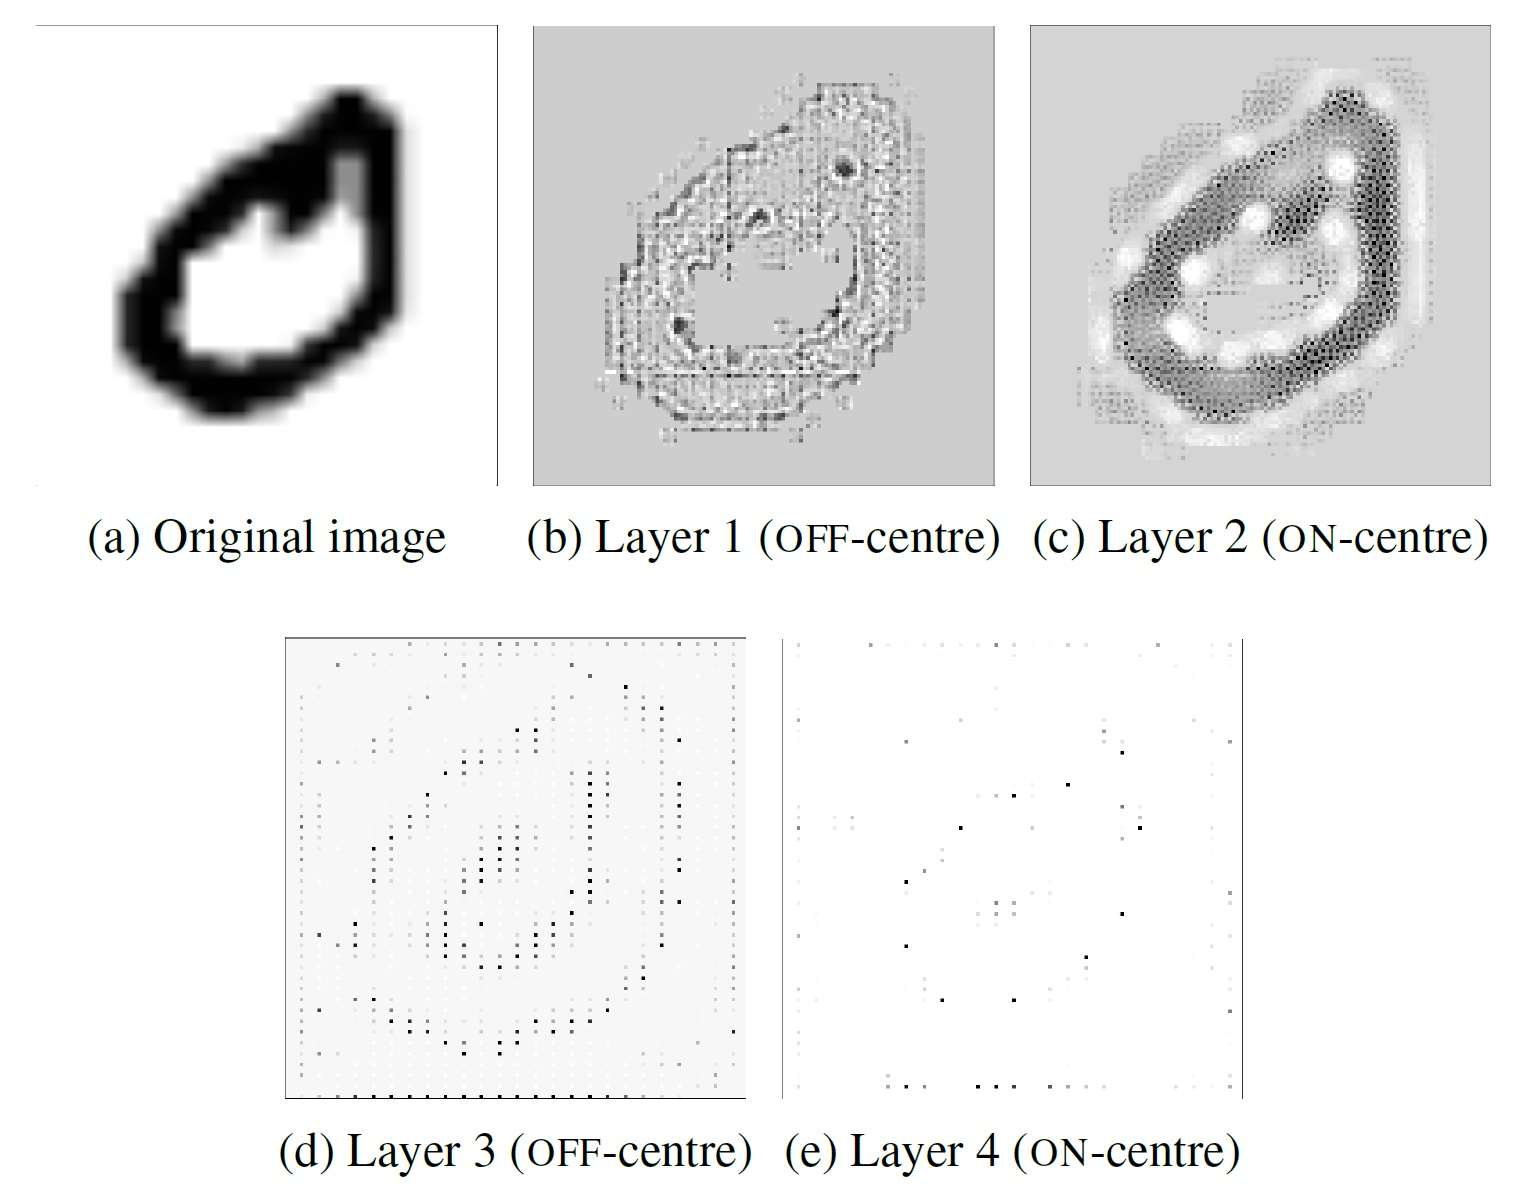
\includegraphics[width=0.8\textwidth]{pics_bench/fig2.jpg}
%	\caption{Results of convolving the image spikes with the simulated ganglion cell layers using the FoCal algorithm before correcting for filter overlap. (a) The original image. (b-e) the result of convolving the image with the layer 1 (smallest) OFF-centre to layer 4 (largest) ON-centre kernels respectively.}
%	\label{fig-convolution-results}
%\end{figure}
%Every pixel value in the convolved image (Figure~\ref{fig-convolution-results}) 
%is inversely proportional to the spike emission time relative to the presentation of the image (i.e. the higher the pixel value, the sooner the spike will fire.)
%
%Since DoGs are used as the means to encode the image, and they do not form an orthogonal set of basis functions, the algorithm also performs a redundancy correction step.
%It does so by adjusting the convolved images' pixel values according to the correlation between convolution kernels (Alg.~\ref{code-focal-corr}).
%
%\begin{algorithm}[h]
%	\caption{FoCal, redundancy correction}
%	\label{code-focal-corr}
%	\begin{algorithmic}
%		\Procedure{Correction}{coeffs $C$, correlations $Q$}
%		\State $N \leftarrow \emptyset$ \Comment{Corrected coefficients}
%		\Repeat
%		\State $m \leftarrow max(C)$\Comment{Obtain maximum from $C$}
%		\State $M \leftarrow M \cup m$\Comment{Add maximum to $M$}
%		\State $C \leftarrow C \setminus m$\Comment{Remove maximum from $C$}
%		\ForAll{$ c \in C$} \Comment{Adjust all remaining $c$}
%		\If{$Q(m, c) \neq 0$} \Comment{Adjust only spatially near coefficients}
%		\State $c \leftarrow c - m \times Q(m, c)$
%		\EndIf
%		\EndFor
%		\Until{$C = \emptyset$}
%		\State \textbf{return} $M$
%		\EndProcedure
%	\end{algorithmic}
%\end{algorithm}
%
%
%After the correction step, the most important information can be recovered using only the first 30\% of the spikes~\citep{sen2009evaluating}. These most significant spikes are shown in Figure~\ref{fig-raster-plot-30pc}, which shows the spikes firing at 1~ms intervals. Neurons in Layer 1 emit spikes faster and in larger quantities than any other layer, making it the most important layer. Layers 2 and 3 have few spikes due to the large convolution kernels used to simulate the ganglion cells. One of the main advantages of ROC is that a neuron will only spike once, as can be seen particularly clearly in these two layers. Layers 0 and 1 encode fine detail which can be used to identify what is in the image, while layers 2 and 3 result in blob-like features that should prove useful to location problems.
%
%\begin{figure}[hbt]
%	\centering
%	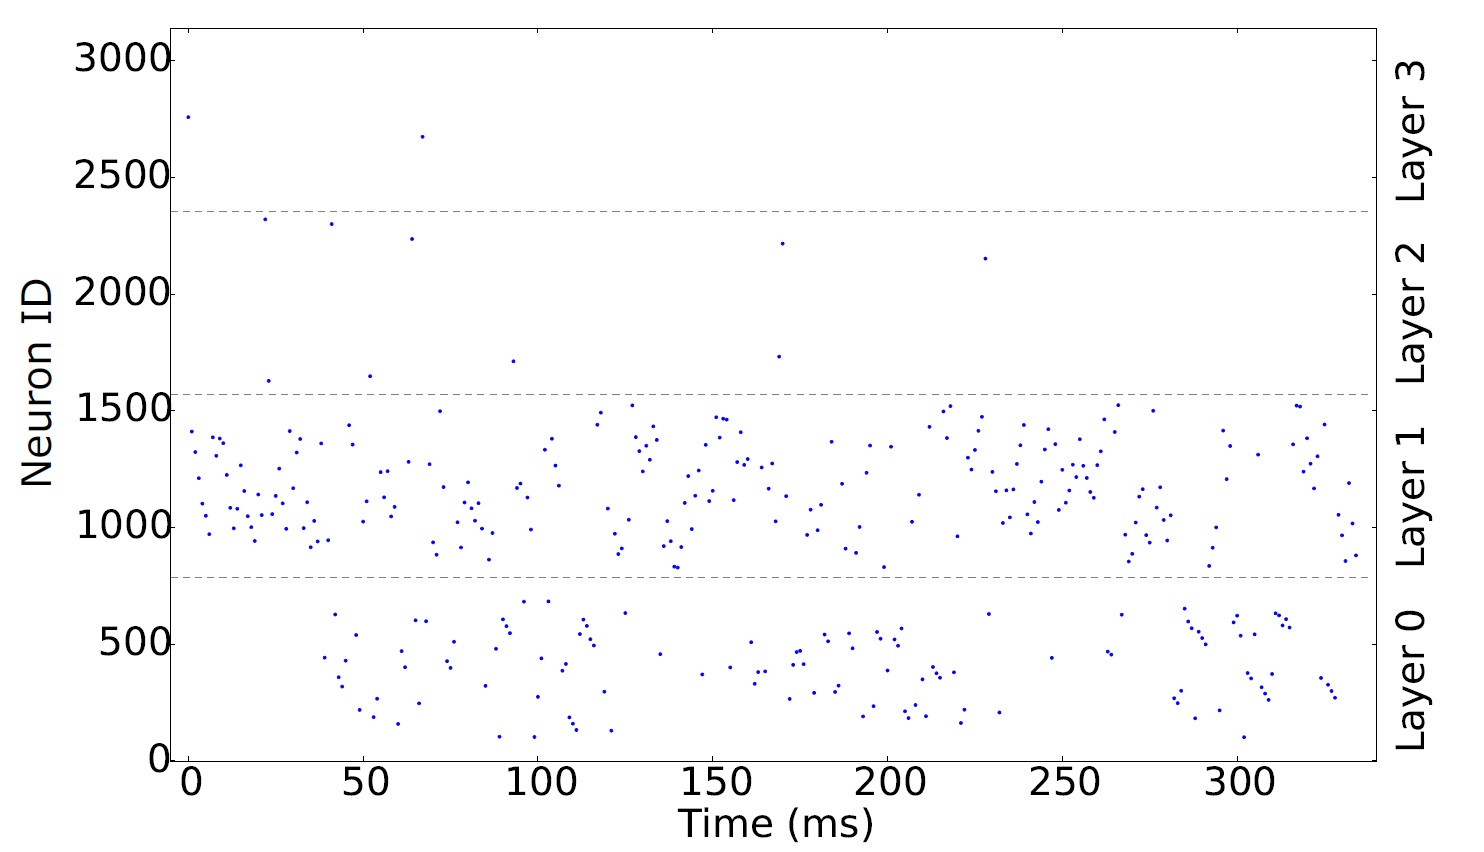
\includegraphics[width=0.8\textwidth]{pics_bench/fig3.jpg}
%	\caption{Raster plot showing the first 30\% of the rank-order encoded spikes produced using FoCal at 1~ms intervals.}
%	\label{fig-raster-plot-30pc}
%\end{figure}
%
%Figure~\ref{fig-reconstruction-results} shows the reconstruction results for the two stages of the algorithm. In Figure~\ref{fig-reconstruction-results}(b) the reconstruction was applied after the convolution but without the FoCal correction; a blurry image is the result of redundancy in the spike representation. A better reconstruction can be obtained after Algorithm~\ref{code-focal-corr} has been applied; the result is shown in Figure~\ref{fig-reconstruction-results}(c).
%
%
%\begin{figure}[hbt]
%	\centering
%	%	\subfloat[Original image]{
%	%		\label{sfig-rank-ordered-original-1}
%	%		\includegraphics[width=0.15\textwidth]{original_21-0}
%	%	}
%	%	\subfloat[No correction]{
%	%		\label{pic-lena-reconstructed-raw}
%	%		\includegraphics[width=0.15\textwidth]{reconstructed_21-0_raw}
%	%	}
%	%	\subfloat[FoCal]{
%	%		\label{pic-lena-reconstructed-focal}
%	%		\includegraphics[width=0.15\textwidth]{reconstructed_21-0_100pc}
%	%	}
%	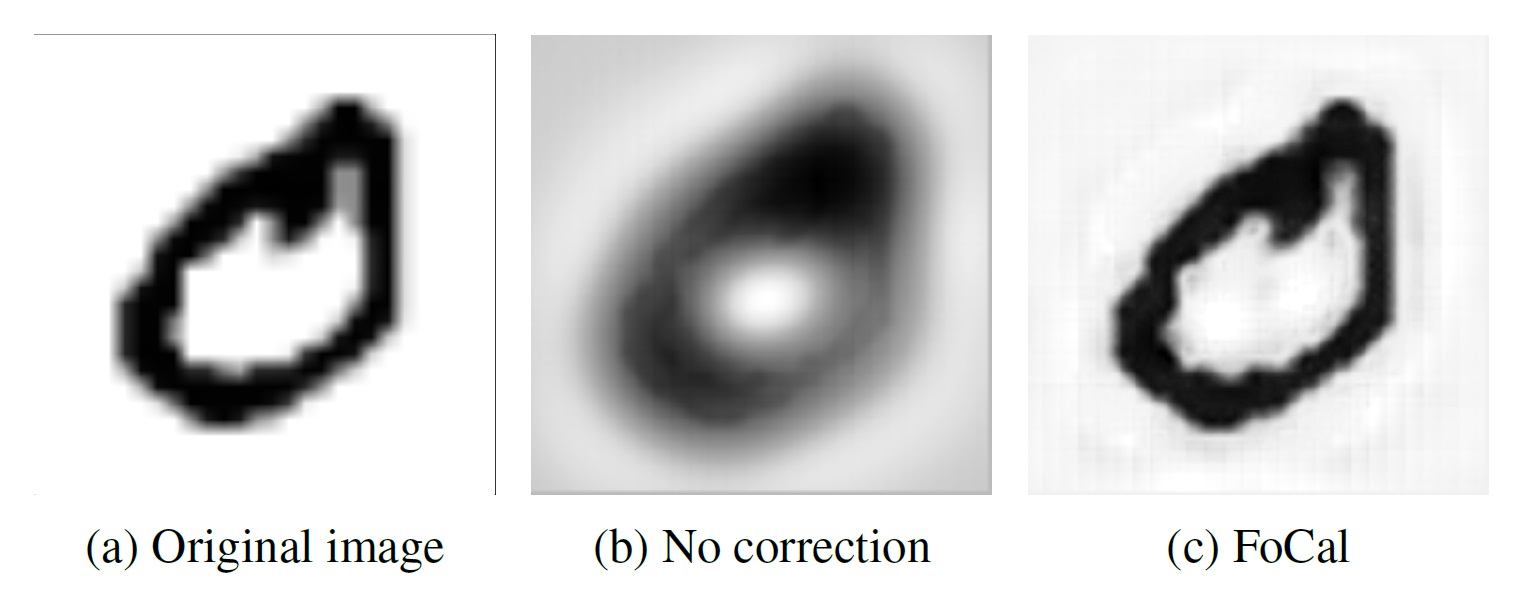
\includegraphics[width=0.8\textwidth]{pics_bench/fig4.jpg}
%	\caption{Reconstruction result comparison. (a) The original image. (b) Reconstruction without overlap correction. (c) Reconstruction with overlap correction.}
%	\label{fig-reconstruction-results}
%\end{figure}
%


\subsubsection{DVS Sensor Output with Flashing Input}
\label{subsec_flash}
The purpose of including the subset with DVS-recorded flashing digits is to promote research into rapid and accurate `core recognition', thus to encourage research into non-rate-based algorithms to shorten the recognition time.

%applying non-rate-based algorithms, for example ROC, to short the DVS output spike trains.

Each digit was shown alternating with a blank image and each display lasted one second.
The digits were displayed on an LCD monitor in front of the DVS retina~\citep{serrano2013128} and were placed in the centre of the visual field of the camera.
Since there are two spike polarities - `ON' indicating an increase in the intensity while `OFF' indicates a decrease - there are `ON' and `OFF' flashing recordings respectively per digit.
In Figure~\ref{fig:flash}, the burstiness of the spikes is illustrated where most of the spikes occur in a 30~ms time slot. 
In total, this subset of the database contains 2$\times$60K recordings for training and 2$\times$10K for testing.

\begin{figure}[tbh!]
	\centering
	%	\subfloat[Spikes recorded in the order of neuron ID during 1s of time.]{
	%		\label{fig:flash_all}
	%		\includegraphics[width=0.48\textwidth]{flash_full}
	%	}
	%	\\
	%	\subfloat[Spikes plotted in the sequence of appearing time during 1s of time. Bursty spikes apeer in slots less than 30~ms. ]{
	%		\label{fig:flash_a}
	%		\includegraphics[width=0.48\textwidth]{flash_full_order}
	%	}
	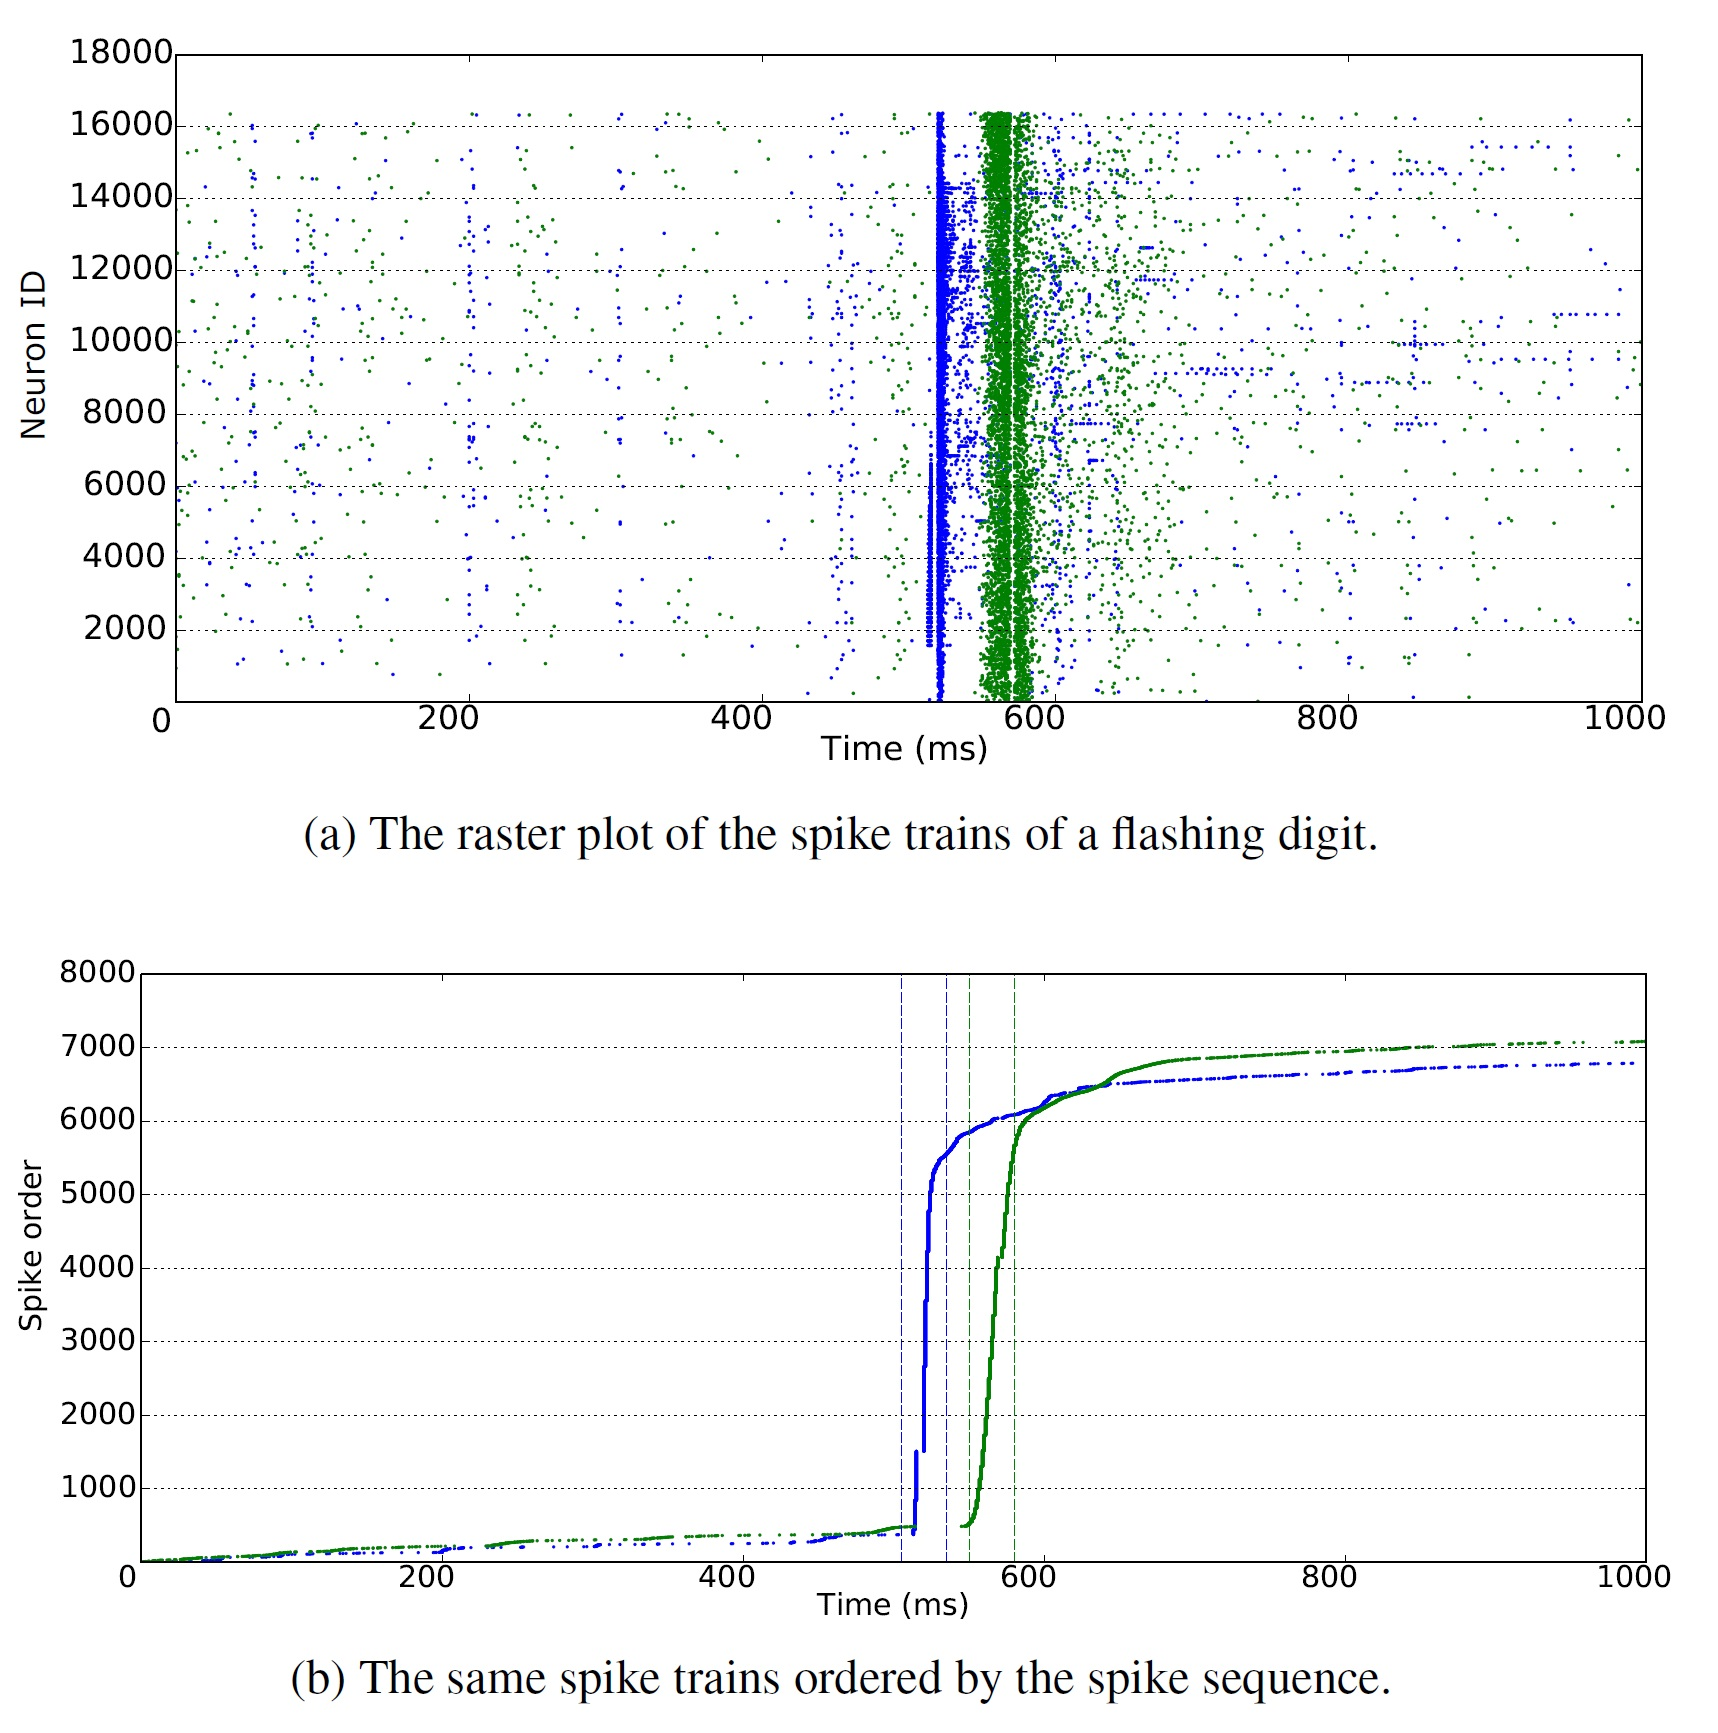
\includegraphics[width=0.8\textwidth]{pics_bench/fig5.jpg}	
	\caption[DVS sensor with flashing input.]{DVS sensor with flashing input.
		Blue is used for `ON' events and green for `OFF' events.
		(a) The raster plot shows spikes generated by individual neurons over time.
		It is hard to recognise the total number of spikes due to the large number of neurons involved in the figure.
		Thus all the spikes are ordered in time, and displayed in the figure below.
		(b) The raster plot shows the ordered spike sequence over time.
		The total number of spikes is around 7K for both `ON' and `OFF' events.
		The bursty nature of the resulting spikes is illustrated, where most of the spikes occur in a 30~ms time slot.}
	\label{fig:flash}
\end{figure}

\subsubsection{DVS Sensor Output with Moving Input}

The subset of DVS recorded moving digits is provided by Teresa~Serrano-Gotarredona, and is  presented to address the challenges of position- and scale- invariance in computer vision.
MNIST digits were scaled to three different sizes, using smooth interpolation algorithms to increase their size from the original 28$\times$28 pixels, and displayed on the monitor with slow motion. 
The same DVS~\citep{serrano2013128} used in Section~\ref{subsec_flash} captured the movements of the digits and generated spike trains for each pixel in its 128$\times$128 resolution.
A total of 30K recordings were made: 10 digits, at 3 different scales, 1K different handwritten samples for each.

\section{Performance Evaluation}
\label{sec:eval}
As a result of the spike-based processing used in SNN models, new concerns about the latency and energy cost arise over performance assessment.
Therefore we propose corresponding evaluation metrics and suggest a sufficient description of SNN models in this section.
Once a model is implemented on a neuromorphic platform, the hardware performance can be evaluated by running the particular model.
This model-specific assessment provides more robust comparisons between hardware platforms by using the same network topology, neuron and synaptic models, and learning rules. 
A complementary evaluation methodology is essential to provide common metrics and assess both the model-level and hardware-level performance.


\subsection{Model-level Evaluation}
\label{subsec:model}

A suggested description of an SNN model is shown in Table~\ref{tb:model_eval} where the performance evaluation metrics are in bold and the SNN specific description is in italics.
Because SNNs introduce the time dimension and spike-based processing, additional performance metrics become relevant in addition to classification accuracy: recognition latency and the number of synaptic events.
%Both of the metrics are proposed according to the biological aspects.

Recognition latency measures how fast spikes are conveyed through the layers of network to trigger the recognition neurons.
\citet{dicarlo2012does} considered the rapid ($<$200~ms) and accurate vision recognition in the brain as the essential problem of object recognition.
For real-time systems with live visual inputs, such as robotic systems, a short response latency helps make fast decisions and take rapid action.
The latency is measured as the time difference between the first spike generated by the output layer and the first spike from the input layer.

%A small number of total synaptic events generated by a recognition task indicates the efficiency of the SNN model.
A spike event is a synaptic operation evoked when one action potential is transmitted through one synapse~\citep{sharp2012power}.
Fewer spike events imply lower overall neural activity and lower energy consumption.
The number of synaptic events can be measured as `Sopbs', synaptic operations per biological second.
%\begin{table*}[hbt!]
%	\caption{SNN descriptions at the model level}
%	\begin{center}
%		\bgroup
%		\def\arraystretch{1.5}
%		\begin{tabular}{ l l l l }
%			\begin{mycell}{3.7cm}Input\end{mycell} & 
%			\begin{mycell}{2.5cm} Network\end{mycell} & 
%			\begin{mycell}{3.5cm} Training \end{mycell} & 
%			\begin{mycell}{5cm} Recognition \end{mycell} \\
%			\hline
%			
%			\begin{leftcell}{3.7cm} - \textit{converting methods}\\- preprocessing \end{leftcell} & % preprocessing
%			\begin{leftcell}{2.5cm} - topology\\- \textit{neuron and synaptic type} \end{leftcell}&  % network
%			\begin{leftcell}{4cm} - supervised or not\\- \textit{learning rule} \\ - \textit{biological training time}\end{leftcell}&  % training
%			\begin{leftcell}{5cm} - \textbf{classification accuracy}\\ - \textbf{\textit{response latency}}\\ - \textbf{\textit{number of synaptic events}} \\ - \textit{biological testing time}\\ - \textit{input spiking rate}  \end{leftcell}% recognition
%		\end{tabular}
%		\egroup
%	\end{center}
%	\label{tb:model_eval}
%\end{table*}

\begin{table*}[hbt!]
	\caption{SNN descriptions at the model level}
	\begin{center}
		\bgroup
		\def\arraystretch{1.5}
		\begin{tabular}{ l l}
%			\begin{rightcell}{3cm} \textbf{SNN}\end{rightcell} & 
%			\begin{leftcell}{5cm}\textbf{Description}\end{leftcell} \\
			\hline
			\begin{rightcell}{3cm}Input\end{rightcell} & 
			\begin{leftcell}{5cm} 
				\textit{converting methods}\\
				preprocessing 
			\end{leftcell} \\
%			\hline
			\begin{rightcell}{3cm} Network\end{rightcell} &
			\begin{leftcell}{5cm}
				topology\\
				\textit{neuron and synaptic type}
			\end{leftcell}\\  % network
%			\hline
			\begin{rightcell}{3cm} Training \end{rightcell} & 
			\begin{leftcell}{5cm}
				supervised or not\\
				\textit{learning rule} \\ 
				\textit{biological training time}
			\end{leftcell}\\  % training
%			\hline
			\begin{rightcell}{3cm} Recognition \end{rightcell} &
			\begin{leftcell}{5cm} 
				\textbf{classification accuracy}\\ 
				\textbf{\textit{response latency}}\\
				\textbf{\textit{number of synaptic events}} \\
				\textit{biological testing time}\\
				\textit{input spiking rate}
			\end{leftcell}\\% recognition
			\hline
		\end{tabular}
		\egroup
	\end{center}
	\label{tb:model_eval}
\end{table*}


Alongside the SNN evaluation metrics, a sufficient description of a network model is required so that other researchers can reproduce it and compare it with other models.
First of all, the input of an SNN model is specified.
The description includes the transformation method for converting raw images to spike trains, and the preprocessing either to images or spikes.
Filtering the raw image may ease the classification/recognition task while adding noise may require more robustness in the model.
Secondly, as with the evaluation of conventional artificial neural networks, a description of the network characteristics provides the basis for the overall performance evaluation.
Sharing the designs not only makes the model reproducible but also inspires fellow scientists to bring new points of view to the problem, generating a positive feedback loop where everybody wins.
The main characteristics include the network topology and the neural and synaptic models.
The network topology defines the number of neurons used for each layer and the connections between layers and neurons.
It is essential to state the types of neural and synaptic model (e.g. current-based LIF neuron) utilised in the network and the parameters configuring them, because neural activities differ significantly between configurations.
Any non-neural classifier, sometimes added to aid the design or enhance the output of the network, must also be specified.
Thirdly, the training procedure determines the recognition capability of a network model.
%A clear distinction should be made between supervised, semi-supervised and unsupervised learning.
Specifying the learning algorithm with its mechanism (supervised, semi-supervised and unsupervised) helps the reader understand the core features of the model.
A detailed description of new spike-based learning rules will be a great contribution to the field due to the present paucity of spatio-temporal learning algorithms.
Most publications reflect the use of adaptations to existing learning rules; details on these modifications should be clear and unambiguous.
In conventional computer vision, the number of iterations of training images presented to the network play an important role.
Similarly, the biological training time determines the amount of information provided for training an SNN.
Finally in the testing phase, as well as the performance evaluation metrics stated above, specific configurations of the input spikes are also essential.
This includes details of the way samples are presented to the network: spiking rates, and biological time per test sample.
The combination of these two factors determines how much information is presented to the network.
%Some work on SNN-based classifications of MNIST is listed in Table~\ref{tb:software_comparison}.
Following the formatted evaluation as in Table~\ref{tb:model_eval}, Table~\ref{tb:software_comparison} lists a few SNN models for MNIST classification, although some details are missing. 
%Most of these reports did not provide sufficiently detailed descriptions of the networks and the models were not completely evaluated in the way that we propose.

\begin{table}[htbp] \small 
	\caption{Model-level comparison}
	\begin{center}
%		\bgroup
		\def\arraystretch{1}
		\begin{tabular}{ l c c c c }
			$ $ &
			\begin{mycell}{2cm} Input\end{mycell} & 
			\begin{mycell}{3cm} Network\end{mycell} & 
			\begin{mycell}{2.5cm} Training \end{mycell} & 
			\begin{mycell}{3cm} Recognition \end{mycell} \\
			\hline
			
			%
			\begin{mycell}{0.5cm}~\citep{brader2007learning} \end{mycell} & 
			\begin{mycell}{2cm} Poisson \end{mycell} & % preprocessing
			\begin{mycell}{3cm} Two layer,\\LIF neurons\\bistable synapse\end{mycell}&  % network
			\begin{mycell}{3cm} Semi-supervised, STDP, calcium LTP/LTD\end{mycell}&  % training
			\begin{mycell}{3cm} 96.5\% \end{mycell} \\% recognition

			%
			\begin{mycell}{0.5cm}~\citep{diehl2015unsupervised} \end{mycell} & 
			\centering Poisson&
			\begin{mycell}{3cm} Two layers, LIF neurons, inhibitory feedback  \end{mycell}& 
			\begin{mycell}{3cm} Unsupervised, WTA, STDP,\\ %adaptive membrane potential, 
				%				$3,000,000$~s of training\\ 
				200K~s times\\ 15 iterations\end{mycell} & 
			\begin{mycell}{3cm} 95\% \end{mycell}\\
			%
%			\begin{mycell}{0.5cm}~\citep{beyeler2013categorization} \end{mycell} & 
%			\begin{mycell}{2cm} Scaling, V1 (edge),\\ Poisson\end{mycell} & % preprocessing
%			\begin{mycell}{3cm} V2 (orientation),\\ and competitive decision, Izhikevich neurons\end{mycell}&  % network
%			\begin{mycell}{3cm} Semi-supervised, STDP, \\ calcium LTP/LTD \end{mycell} &  % training
%			\begin{mycell}{3cm} 91.6\% \\ 300~ms per test \end{mycell} \\% recognition
			
			%
			\begin{mycell}{0.5cm}~\citep{neftci2013event} \end{mycell} & 
			\begin{mycell}{2cm} Thresholding, Poisson\end{mycell} & %  ,\\ Synaptic current
			\begin{mycell}{3cm} Two layers, \\RBM, \\ LIF neurons \end{mycell}&  % network
			\begin{mycell}{3cm} Event-driven contrastive divergence (eCD), unsupervised \end{mycell}&  % training
			\begin{mycell}{3cm} 91.9\% \\ 1~s per test\end{mycell} \\% recognition
			
			\begin{mycell}{0.5cm}~\citep{neftci2016stochastic} \end{mycell} & 
			\begin{mycell}{2cm} Thresholding, Poisson\end{mycell} & % preprocessing Thresholding,\\ Synaptic current
			\begin{mycell}{3cm} Two layers,\\RBM, \\ LIF neurons \end{mycell}&  % network
			\begin{mycell}{3cm} Synaptic Sampling Machine + eCD, unsupervised \end{mycell}&  % training
			\begin{mycell}{3cm} 95.8\% \\ 250~ms per test\end{mycell} \\% recognition
			%
			\begin{mycell}{0.5cm} % %\citep{Stromatias2015scalable} \\ 
				\citep{stromatias2015robustness} \end{mycell} & 
			\begin{mycell}{2cm} Poisson \end{mycell} & % preprocessing
			\begin{mycell}{3cm} Four layers, \\RBM, \\ LIF neurons \end{mycell}&  % network
			\begin{mycell}{3cm} Off-line trained, unsupervised \end{mycell}&  % training
			\begin{mycell}{3cm} 94.94\%\\16 ms latency \\ 1.44M Sopbs\end{mycell} \\% recognition
			
			%
			\begin{mycell}{0.5cm}~\citep{diehl2015fast}\end{mycell}& 
			\begin{mycell}{2cm}Poisson\end{mycell} & % preprocessing
			\begin{mycell}{3cm} Six layers,\\ConvNet, \\IF neurons\end{mycell}& % network
			\begin{mycell}{3cm} Off-line trained with ReLU, weight normalisation \end{mycell}&   % training
			\begin{mycell}{3cm} 99.1\%, \\0.5~s per test\end{mycell}\\ % recognition    
			%
			\begin{mycell}{0.5cm}~\citep{zhao2014feedforward}\end{mycell}  & 
			\begin{mycell}{2cm} Thresholding \\ or DVS \end{mycell}& % preprocessing 
			\begin{mycell}{3cm} Simple (Gabor), \\Complex (MAX) \\and Tempotron  \end{mycell}& % network
			\begin{mycell}{3cm} Tempotron, supervised \end{mycell}& % training
			\begin{mycell}{3cm} 91.3\%(Thresholding)\\ 11~s per test \\ 88.1\%(DVS),\\ 2~s per test\end{mycell}\\ % recognition
			
			\begin{mycell}{0.5cm}Chpt4\end{mycell}& 
			\begin{mycell}{2cm}Poisson\end{mycell} & % preprocessing
			\begin{mycell}{3cm} Six layers,\\ConvNet, \\LIF neurons\end{mycell}& % network
			\begin{mycell}{3cm} Off-line trained with ReLU,\\ Noisy Softplus fine-tune\end{mycell}&   % training
			\begin{mycell}{3cm} 99.07\%, \\1~s per test\\35.24~ms\\$53.4$M Sopbs\end{mycell}\\ % recognition    
			
			\begin{mycell}{0.5cm}Chpt5\end{mycell}& 
			\begin{mycell}{2cm}Poisson\end{mycell} & % preprocessing
			\begin{mycell}{3cm} Two layers,\\ Autoencoders~(AE), \\LIF neurons\end{mycell}& % network
			\begin{mycell}{3cm} Event-driven, spike-based AE\\18K~s training, unsupervised\end{mycell}&   % training
			\begin{mycell}{3cm} 94.72\%, \\1~s per test\\21.68~ms\\$5.26$M Sopbs\end{mycell}\\ % recognition    
			%
			\begin{mycell}{0.5cm} Case Study \end{mycell}  & 
			\begin{mycell}{2cm} Poisson \end{mycell}& % preprocessing 
			\begin{mycell}{3cm} Fully connected decision layer, \\ LIF neurons \end{mycell}& % network
			\begin{mycell}{3cm} K-means clusters,\\Supervised STDP\\18K~s of training \end{mycell}& % training
			\begin{mycell}{3cm} 92.99\%\\1~s per test \\13.82~ms latency\\$4.17$M Sopbs\end{mycell}\\ % recognition
		\end{tabular}
%		\egroup
	\end{center}
	\label{tb:software_comparison}
\end{table}

\subsection{Hardware-level Evaluation}
\label{subsec:hw}

\begin{sidewaystable*}[htbp] \small
	\caption{Hardware-level comparison}
	\begin{center}
		\begin{minipage}{\textwidth}
			
			\begin{savenotes}
				\bgroup
				\def\arraystretch{1.4}
				\begin{tabular}{l c c c c c c}
					$ $ & 
					\begin{mycell}{2.0cm} System \end{mycell} & 
					%       \begin{minipage}{1.3cm}\centering Simulation type \end{minipage} & 
					
					\begin{mycell}{4.0cm} Neuron Model \end{mycell} & 
					\begin{mycell}{2.0cm}Synaptic\\Plasticity\end{mycell} &
					%       \begin{minipage}{1cm}\centering Axonal delays \end{minipage} & 
					%       \begin{minipage}{1cm}\centering Synaptic model \end{minipage} & 
					\begin{mycell}{2.0cm} Precision \end{mycell} &  
					%       \begin{minipage}{1.2cm}\centering Synaptic precision \end{minipage} & 
					%       \begin{minipage}{1.2cm}\centering Energy per SE \end{minipage} & 
					%       \begin{minipage}{1.4cm}\centering Synaptic ops per Watt \end{minipage} & 
					\begin{mycell}{2.0cm} Simulation\\Time \end{mycell} & 
					\begin{mycell}{2.0cm} Energy \\Usage \end{mycell} 
					%       \begin{minipage}{1.7cm}\centering Programming front-end \end{minipage}  
					\\
					\hline
					% contents!
					
					\begin{mycell}{1.8cm} SpiNNaker \citep{stromatias2013power} \end{mycell} &
					\begin{mycell}{2.0cm} Digital, \\Scalable \end{mycell} & 
					\begin{mycell}{4.0cm}Programmable\\Neuron and Synapse,\\Axonal delay \end{mycell}& 
					\begin{mycell}{2.0cm}Programmable\\learning rule\end{mycell}& 
					\begin{mycell}{2.0cm}11- to 14-bit synapses\end{mycell} & 
					\begin{mycell}{2.0cm} Real-time \\ Flexible time resolution \end{mycell}  &
					\begin{mycell}{2.5cm} 8~nJ/SE \end{mycell} \\
					%
					\begin{mycell}{1.8cm} TrueNorth \citep{merolla2014million}\end{mycell} & \begin{mycell}{2.0cm}Digital, \\Scalable \end{mycell}& 
					\begin{mycell}{4.0cm}Fixed models,\\Config params,\\Axonal delay\end{mycell}& 
					\begin{mycell}{2.0cm}No plasticity\end{mycell}& 
					\begin{mycell}{2.2cm}122 bits \\params \& states,
						%       	 per neuron
						\\4-bit/\\4 values\\synapses\footnotemark[1]
					\end{mycell}& 
					\begin{mycell}{2.0cm}Real-time\end{mycell}& 
					\begin{mycell}{2.0cm}26 pJ/SE\end{mycell} \\
					
					%
					\begin{mycell}{1.8cm} Neurogrid \citep{benjamin2014neurogrid}\end{mycell} &
					\begin{mycell}{2.0cm}Mixed-mode,\\Scalable\end{mycell} & 
					\begin{mycell}{4.0cm}Fixed models,\\Config params\end{mycell} & 
					\begin{mycell}{2.0cm}Fixed rule\end{mycell} & 
					\begin{mycell}{2.0cm}13-bit shared \\ synapses\end{mycell} &
					\begin{mycell}{2.0cm}Real-time\end{mycell} &
					\begin{mycell}{2.0cm}941 pJ/SE\end{mycell} \\
					%
					\begin{mycell}{1.8cm} HI-CANN \citep{schemmel2010wafer}  \end{mycell} & \begin{mycell}{2.0cm}Mixed-mode,\\Scalable\end{mycell} &
					\begin{mycell}{4.0cm}Fixed models,\\Config params\end{mycell}& 
					\begin{mycell}{2.0cm}Fixed rule\end{mycell}& 
					\begin{mycell}{2.0cm}4-bit/\\16 values\\synapses\end{mycell}& 
					\begin{mycell}{2.0cm}Faster than\\ real-time\footnotemark[2]
					\end{mycell}&
					\begin{mycell}{2.0cm} 7.41 nJ/SE\\(network only) \end{mycell}\\
					%
					\begin{mycell}{1.8cm} HiAER-IFAT \citep{yu201265k}\end{mycell} & 
					\begin{mycell}{2.0cm}Mixed-mode,\\Scalable\end{mycell} &
					\begin{mycell}{4.0cm}Fixed models,\\Config params\end{mycell}& 
					\begin{mycell}{2.0cm}No plasticity\end{mycell} &  
					\begin{mycell}{2.0cm}Analogue neuron/synapse\end{mycell} & 
					Real-time&
					\begin{mycell}{2.0cm}22-pJ/SE\\\citep{park201465k}\end{mycell}
					
					%dummy update text
				\end{tabular}
				\egroup
				
			\end{savenotes}
		\end{minipage}
	\end{center}
	\label{tb:hardware_comparison}
	\footnotetext[1]{We consider them 4-bit synapses because it is only possible to choose between 4 different signed integers and whether the synapse is active or not.}
	\footnotetext[2]{A maximum speed-up of up to $10^5$ times real time has been reported.}
\end{sidewaystable*}


A direct comparison between neuromorphic platforms is a non-trivial task due to the different hardware implementation technologies as mentioned in Section~\ref{subsec:neuromorphic_hw}.
%Qian Liu modified
Table~\ref{tb:hardware_comparison} attempts to describe the neuromorphic hardware platforms with reference to different aspects of SNN simulation.
The scalability of a hardware platform determines the network size limit of a neural application running on it.
Considering the various neural and synaptic models, plasticity learning rules and lengths of axonal delays, a programmable platform offers flexibility to support diverse SNNs while a hard-wired system supporting only specific models is advantageous due to its energy-efficiency and simpler design and implementation.
The classification accuracy of an SNN running on a hardware system can be different from the software simulation, since hardware implementations may impose limits on the precision used for the membrane potentials of neurons (for the digital platforms) and the synaptic weights.
%Thus comparison metrics is supposed to include precision as a major assessment of the system performance.
Simulation time is another important measure when running large-scale networks on hardware.
Real-time implementation is an essential requirement for robotic systems because of the real-time input from the neuromorphic sensors.
Running faster than real time is attractive for large and long simulations.
%Finer time resolution plays an important role in precision-sensitive neural models or in sub-millisecond tasks~\citep{lagorce2015breaking}.
%Qian Liu done
It is interesting to compare the performance of each platform in terms of energy requirements, especially if the platform targets mobile applications and robotics.
Some researchers have suggested the use of energy per synaptic event (J/SE)~\citep{sharp2012power,stromatias2013power} as an energy metric because the large fan in and out of a neuron means that synaptic processing tends to dominate the total energy dissipation during a simulation.
\citet{merolla2014million} proposed the number of synaptic operations per second per Watt (Sops/W).
These two measures are equivalent, since J/SE$\times$Sops/W = 1.
%To investigate the power usage in detail, \citep{Diamond2016comparing} included the power drawn by the attached workstations.
%This work indicated the power variation by each task over time.

%Qian Liu modified
However, the typical reported simulation time and energy use for the various platforms is under different SNN models, making the comparisons problematic.
Model-specific hardware metrics would provide robust comparisons between platforms and expose how different networks influence the metrics on particular hardware.
The proposed evaluation metrics consist of the \textbf{feasibility}, \textbf{classification accuracy}, \textbf{simulation time} and \textbf{energy use}.
A particular SNN model is feasible to run on a particular hardware platform only when the network size is under the platform's limit, the neural and synaptic models are supported, and the learning rule is implemented.
CA also plays a role in hardware evaluation because of the precision limits that may be imposed by the platform.
Due to the limited hardware resources, simulation time may accelerate or slow down according to the network topology and spike dynamics.
Similarly, energy costs vary with different networks and neural and synaptic models.
%The system performance will be assessed on the accuracy, simulation time and energy use running the network. 
%Table~\ref{tb:hardware_comparison} aims to summarise the aforementioned hardware comparison metrics.
%\begin{table*}[hbt!]
%	\caption{Hardware level evaluation of model specific SNN simulation}
%	\begin{center}
%		\bgroup
%		\def\arraystretch{1.5}
%		\begin{tabular}{ l l l l }
%			\begin{mycell}{5cm} Hardware Description \end{mycell} & 
%			\begin{mycell}{5cm} Evaluation Metrics \end{mycell} \\
%			\hline
%			\begin{leftcell}{5cm} - Digital/Analogue \\- Scalability\\- Neuron models supported\\- Synapse models supported\\- Synaptic plasticity \\- Precision \end{leftcell}&  % training
%			\begin{leftcell}{5cm} - feasibility\\- classification accuracy \\- simulation time \\- energy use \end{leftcell}% recognition
%		\end{tabular}
%		\egroup
%	\end{center}
%	\label{tb:hw_eval}
%\end{table*}

\section{Results}
\label{sec:test}
In this section, we present a recognition SNN model working on the Poissonian subset of the NE15-MNIST dataset.
The network components, training and testing methods are described along the lines set out in Section~\ref{subsec:model}.
The recognition result is evaluated using the proposed metrics: classification accuracy, response latency and number of synaptic events.
%The specific spike-based evaluations on input event rates and/or responding latency are also provided. 
As tentative benchmarks the models are implemented on SpiNNaker to assess the hardware-level performance against software simulators.
Presenting proper benchmarks for vision recognition systems is still under investigation; the case study only make a first attempt.

%\subsection{Case Study I}
The case study is a simple two-layer network where the input neurons receive Poisson spike trains from the dataset and form a fully connected network with the decision neurons.
There is at least one decision neuron per digit to classify a test input.
The neuron with the highest output firing rate classifies a test image as the digit it represents.
The model utilises LIF neurons, and the parameters are all biologically valid, see the listed values in Table~\ref{tbl:pynnSetting}.
The LIF neuron model follows the membrane potential dynamics~(Equation~\ref{equ:LIF_V}):

\begin{equation}
\tau_m \frac{\D V}{\D t}=V_{rest} - V + R_{m} I(t) ~~~,
\label{eq:LIF}
\end{equation}

where $\tau_m$ is the membrane time constant, $ V_{rest} $ is the resting potential, $ R_{m} $ is the membrane resistance and $ I $ is the synaptic input current.
In PyNN, $ R_{m} $ is represented by $ R_{m}=\tau_m/C_{m} $, where $C_{m} $ is the membrane capacitance.
A spike is generated when the membrane potential goes beyond the threshold, $ V_{thresh} $ and the membrane potential then resets to $V_{reset}$.
In addition, a neuron cannot fire within the refractory period, $ \tau_{refrac} $, after generating a spike.

The connections between the input neurons and the decision neurons are plastic, so the connection weights can be modulated during training with a multiplicative STDP learning rule, refer to Section~\ref{subsec:STDP} for more detail.
The model is described with PyNN and the code is published in
%\footnote {https://github.com/qian-liu/benchmarking/tree/master/code/case\_study\_I}
the Github repository with the dataset.
As a potential benchmark, this system is composed of simple neural models, trained with standard learning rules and written in a standard SNN description language. These characteristics allow the same network to be tested on various simulators, both software- and hardware-based.

Both training and testing use the Poissonian subset of the NE15-MNIST dataset.
This makes performance evaluation on different simulators possible with the unified spike source array provided by the dataset. 
In terms of this case study, the performance of the model was evaluated with both software simulation (on NEST~\citep{gewaltig2007nest}) and on a hardware implementation (on SpiNNaker).

In order to fully assess the performance, different settings were configured on the network, such as network size, input rate and test image duration.
For simplicity of describing the system, a set of standard configuration is used as the example in the following sections.

\begin{table}[hbbp]
	\centering
	\caption[LIF parameter setting using PyNN.]{Parameter setting for the current-based LIF neurons using PyNN.}
	\bgroup
	\def\arraystretch{1.4}
	\begin{tabular}{c c c}
		%\hline
		Parameters & Values & Units \\
		\hline
		cm & 0.25 & nF	\\
		%\hline
		tau\_m & 20.0 & ms\\
		%\hline
		tau\_refrac & 2.0 & ms\\
		%\hline
		%  tau\_syn\_E & 1.0 & ms\\
		%  %\hline
		%  tau\_syn\_I & 1.0 & ms\\
		%  %\hline
		v\_reset & -70.0 & mV\\
		%\hline
		v\_rest & -65.0 & mV\\
		%\hline
		v\_thresh & -50.0 & mV\\
		%\hline
	\end{tabular}
	\egroup
	\label{tbl:pynnSetting}
\end{table}

\subsection{Training}
There are two layers in the model: 28$\times$28 input neurons fully connect to 100 decision neurons.
Each decision neuron responds to a certain digit template.
In the standard configuration, there are 10 decision neurons responding to each digit with slightly different templates.
Those templates are embedded in the connection weights between the two layers.
Figure~\ref{fig:model}(a) shows how the connections to a single decision neuron are tuned.

\begin{figure}[thb!]
	\centering
	%	\subfloat[Training model of a single decision neuron.]{
	%		\label{Fig:train}
	%		\includegraphics[width=0.48\textwidth]{training}
	%	} \\
	%	
	%	\centering
	%	
	%	\subfloat[Testing model of the spiking neural network.]{
	%		\label{Fig:test}
	%		\includegraphics[width=0.48\textwidth]{testing}
	%	}
	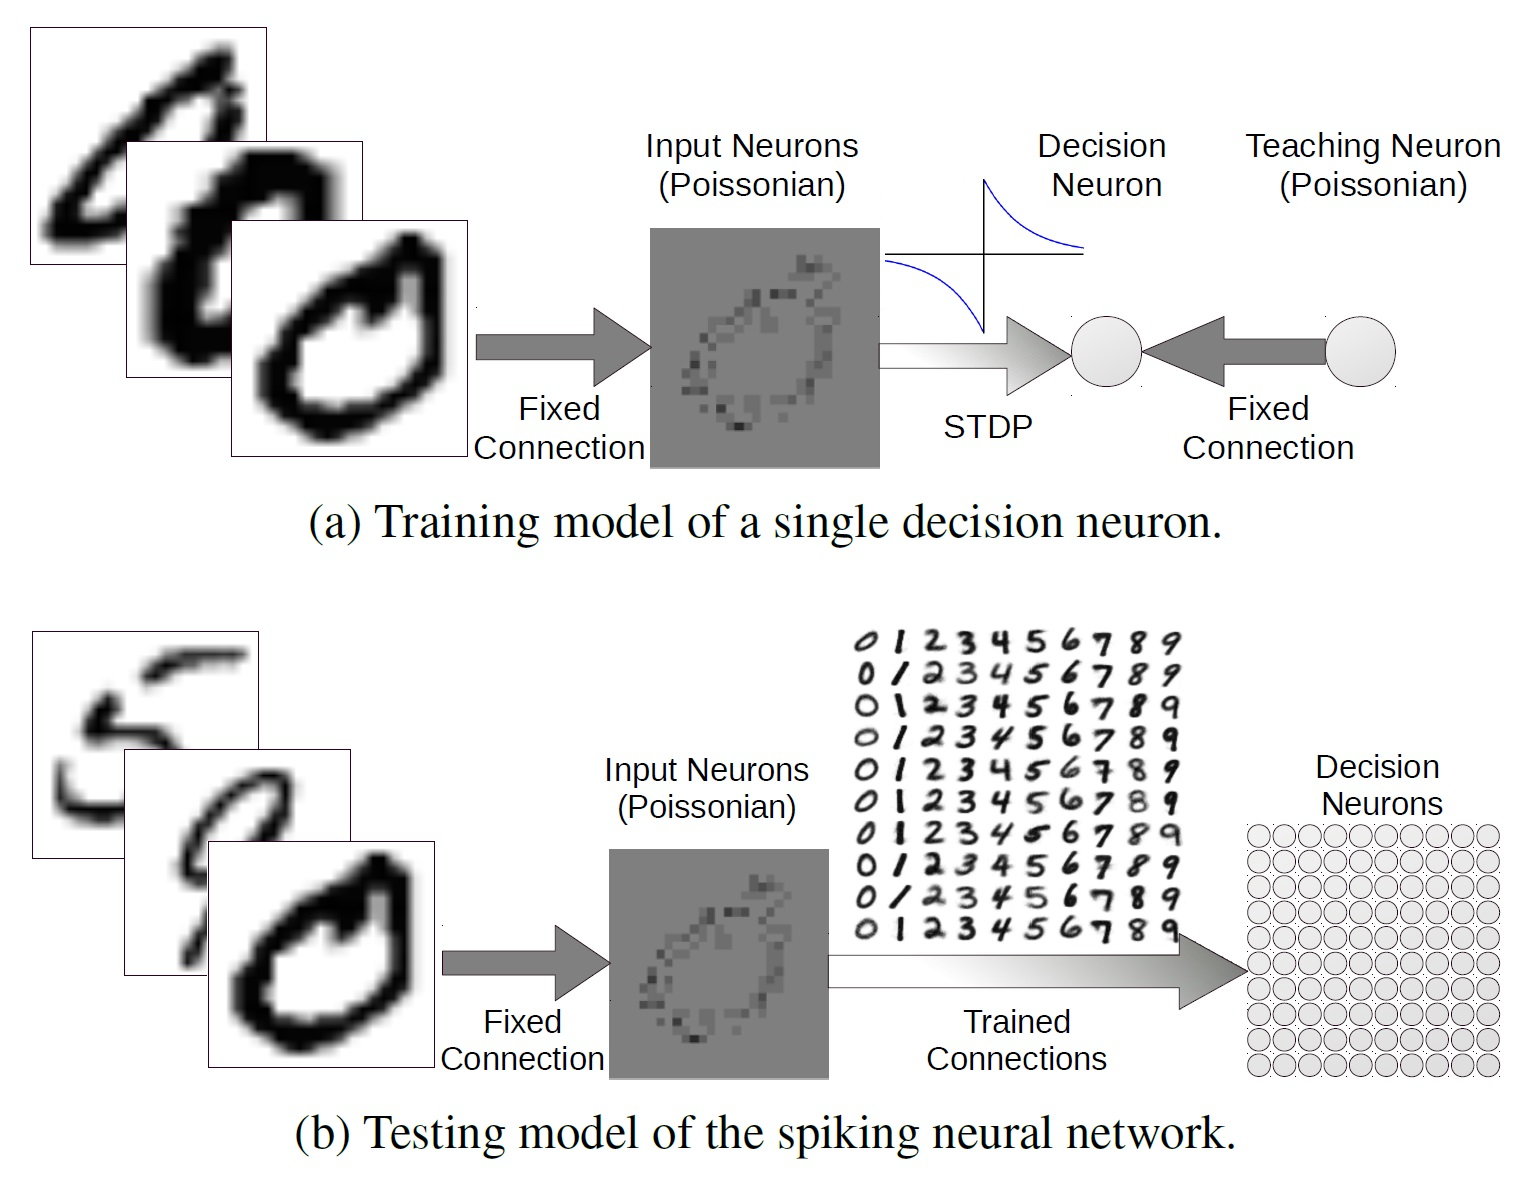
\includegraphics[width=0.7\textwidth]{pics_bench/fig6.jpg}
	\caption[SNN model of the case study.]{The (a) training and (b) testing model of the proposed case study SNN: STDP learning with supervised teaching signal.}
	\label{fig:model}
\end{figure} 

The training set of 60K hand written digits are firstly classified into 100 classes, 10 subclasses per digit, using K-means clusters.
K-means clustering separates a set of data points into K subsets (clusters) according to the Euclidean distance between them.
Therefore each cluster tends to form a boundary within which the data points are near to each other.
In this case, all the images of the same digit (a class) are divided into 10 subclasses by assigning K=10.
Then the images in a certain subclass are used to train a template embedded in the synaptic weights to the corresponding decision neuron.
The firing rates of the input neurons are assigned linearly according to their intensities and the total firing rate of all the 28$\times$28 input neurons is normalised to 2K~Hz, that is, the sum of the firing rates of all of the input neurons is 2K~Hz.
All the images together are presented for 18K~s (about 300~ms per image) during training and at the same time a teaching signal of 50~Hz is conveyed to the decision neuron to trigger STDP learning.
The trained weights are plotted in accordance with the positions of the decision neurons in Figure~\ref{fig:model}(b).





\subsection{Testing}
After training the weights of the plastic synapses are set to static, keeping the state of the weights at the last moment of training.
%The weak weights were set to inhibitory connections with identical strengths in testing.
%The negative connections reduced the output firing rates while keeping a good classification ability.
However, during training the synaptic plasticity holds a hard limit of 0 on the weight strength, thus excitatory synapses cannot change into inhibitory.
To investigate how inhibitory connections influence the classification performance, the weak weights were set to negative with identical strengths.
Results show that inhibitory synapses significantly reduced the output firing rates while keeping a good classification ability.
Thus the strategy of replacing weak weights to the same negative values was used throughout the case study.

The feed-forward testing network is shown in Figure~\ref{fig:model}(b) where Poisson spike trains are generated the same way as in the training with a total firing rate of 2K~Hz per image.
The input neurons convey the same spike trains to every decision neuron through its corresponding trained synaptic weights. 
One test trial contains 10K images in total and each image is presented once and lasts 1~s with a 0.2~s blank period between consecutive images.
The output neuron with the highest firing rate determines which digit is recognised.
With the standard training configuration, we compared the CA of different simulations of the same SNN model.
Using the trained weights from the NEST simulation, the accuracy of the recognition on NEST reached 90.03\%, and this accuracy was also achieved on SpiNNaker.
When the network was both trained and tested on SpiNNaker the recognition accuracy was 87.41\%.
Using these weights in NEST yielded a similar result (87.25\%). 
The reduction in CA using the SpiNNaker trained weights was due to precision loss caused by the limited fast memory and the necessity for fixed-point arithmetic to ensure real-time operation.
It is inevitable that numerical precision will be below IEEE double precision at various points in the processing chain from synaptic input to membrane potential.
The main bottleneck is currently in the ring buffer where the total precision for accumulated spike inputs is 16-bit, meaning that individual spikes are realistically going to be limited to 11- to 14-bit depending upon the probabilistic headroom calculated as necessary from the network configuration and spike throughput~\citep{Hopkins2015Accuracy}.

\subsection{Evaluation}
Evaluation starts from the model-level, focusing on the spike-based recognition analysis.
As mentioned in Section~\ref{subsec:model}, CA, response time (latency) and the total number of synaptic events are the main concerns when assessing the recognition performance.
In our experiment, two sets of weights were applied: the original STDP trained weights, and the scaled-up weights which are 10 times stronger.
The spike rates of the test samples were also modified, ranging from 10 to 5K~Hz.
\begin{figure}[htb!]
	\centering
	%	\subfloat[Accuracy changes against test time.]{
	%		\label{fig:acc_time}
	%		\includegraphics[width=0.25\textwidth]{images/acc_dur}
	%	}
	%	\subfloat[Accuracy changes against firing rate.]{
	%		\label{fig:acc_rate}
	%		\includegraphics[width=0.25\textwidth]{images/acc_rate}
	%	}
	%	\\
	%	\subfloat[Latency stablises against test time.]{
	%		\label{fig:lat_time}
	%		\includegraphics[width=0.25\textwidth]{images/lat_dur}
	%	}
	%	\subfloat[Latency changes against firing rate.]{
	%		\label{fig:lat_rate}
	%		\includegraphics[width=0.25\textwidth]{images/lat_rate}
	%	}
	%	\\
	%	\subfloat[Event rate stablises against test time.]{
	%		\label{fig:eve_time}
	%		\includegraphics[width=0.25\textwidth]{images/time-event}
	%	}
	%	\subfloat[Event rate against firing rate.]{
	%		\label{fig:eve_rate}
	%		\includegraphics[width=0.25\textwidth]{images/rate-event}
	%	}
	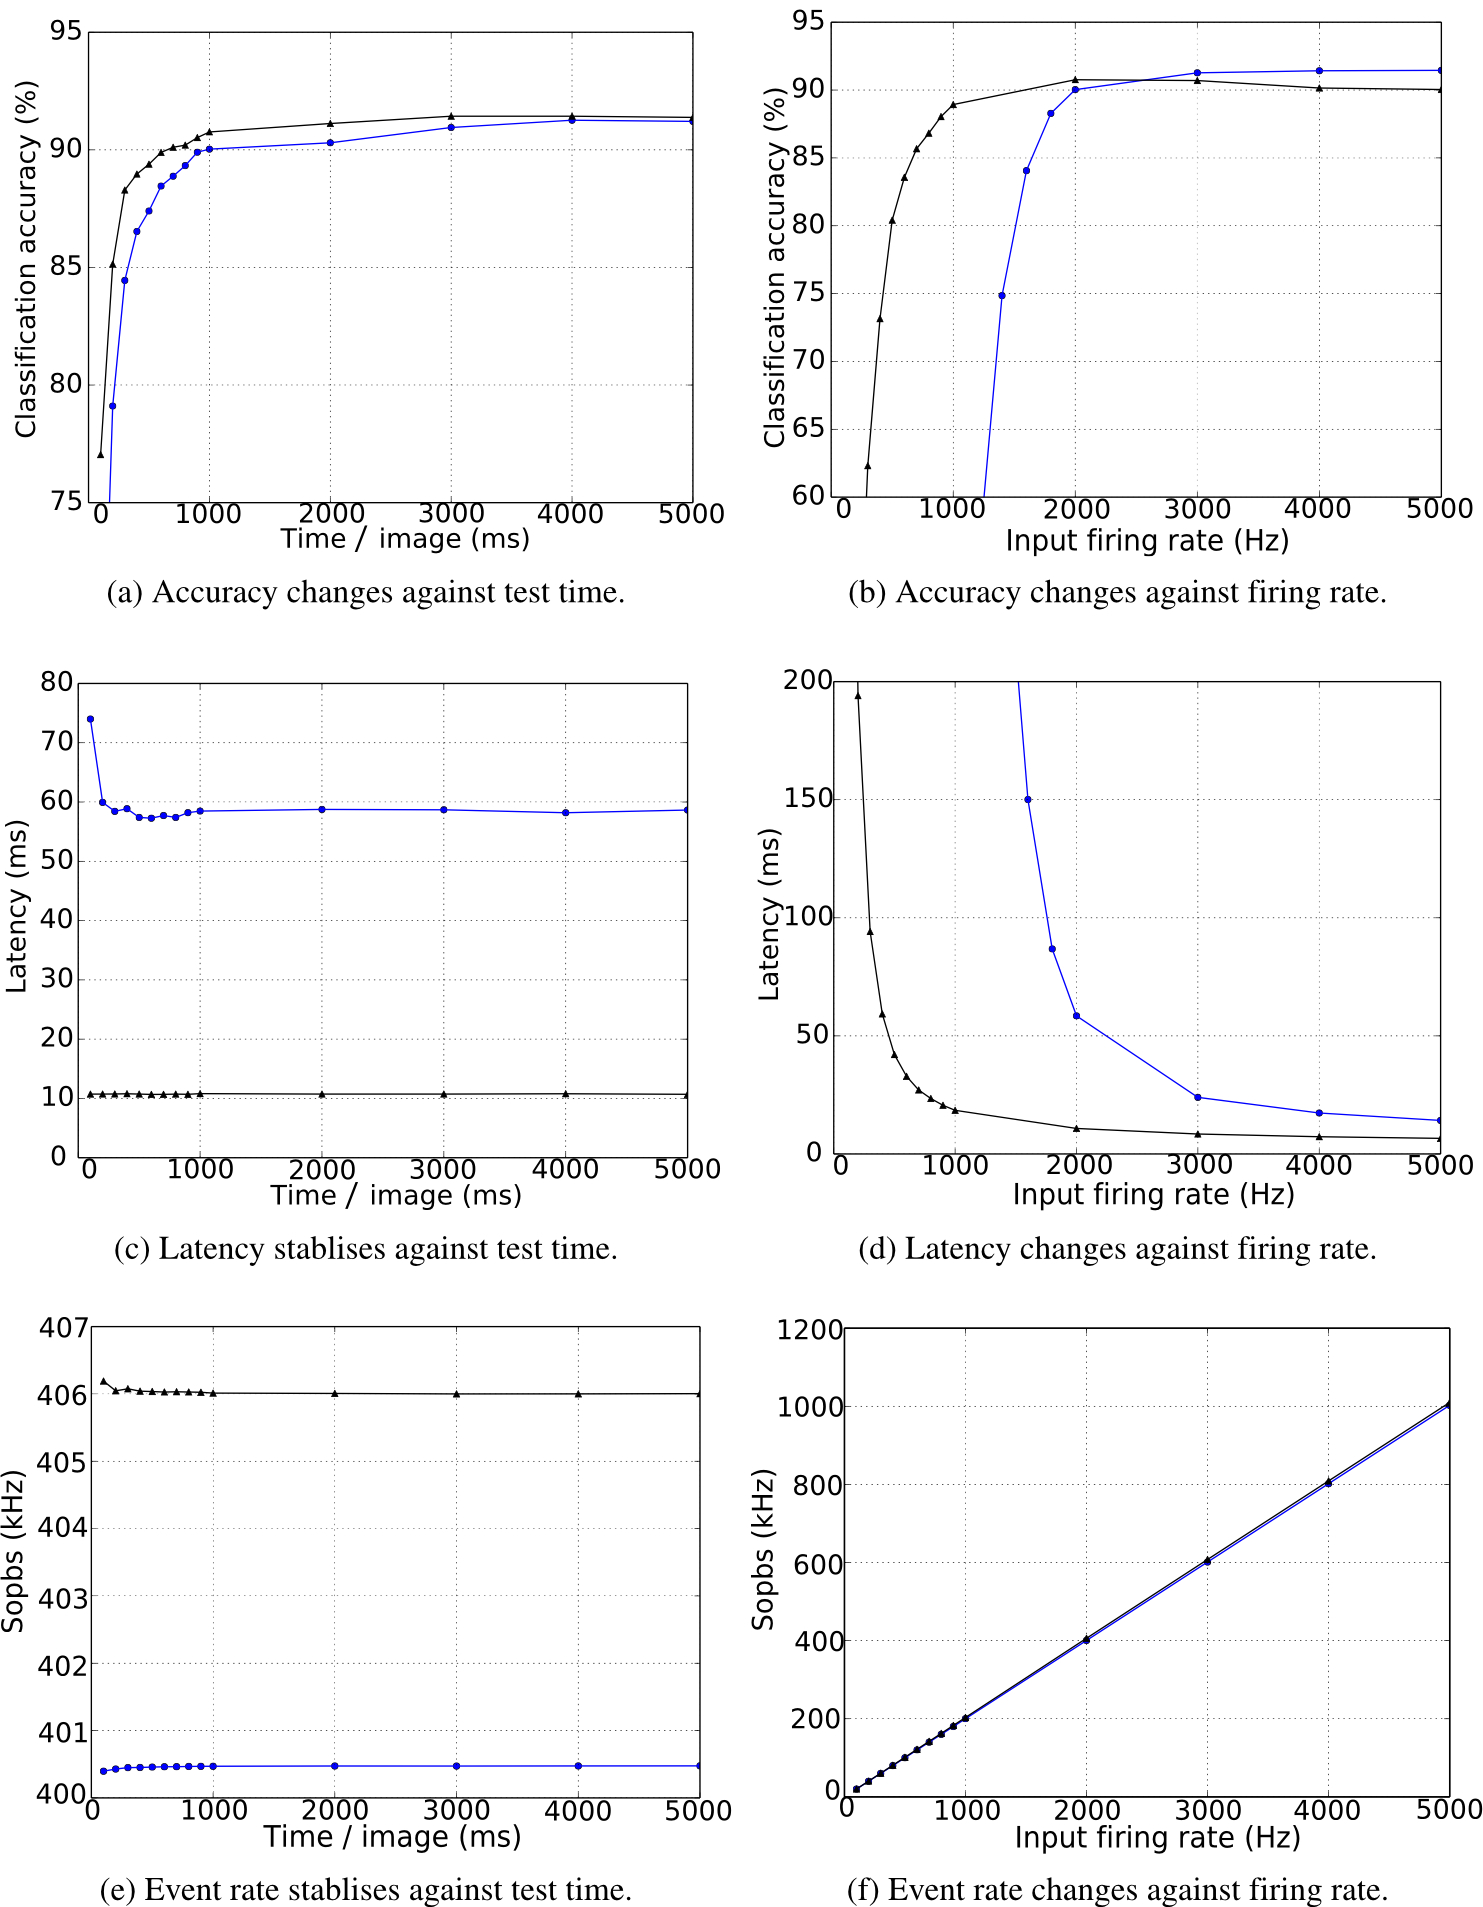
\includegraphics[width=1\textwidth]{pics_bench/fig7.jpg}
	\caption[Comparisons on different test time and input firing rate.]{Accuracy, response time (latency) and synaptic event rate (Sopbs) change over test time and input firing rate per test image.
		The test time is the duration of the presence of a single test image, and the input firing rate is the summation of all the input neurons.
		Original trained weights are used (up-pointing triangles with solid line) as well as the scaled up ($\times10$) weights (down-pointing triangles with dashed line). }
	\label{fig:assess}
\end{figure}

We found that accuracy depends largely on the time each sample is exposed to the network and the sample spike rate (Figure~\ref{fig:assess}).
%Furthermore, the latency of the output of the decision neurons is affected by both the spiking rate and connection weights.
Figure~\ref{fig:assess}(a) shows that the CA is better as exposure time increases. The longer an image is presented, the more information is gathered by the network, so the accuracy climbs.
Classification accuracy also increases when input spike rates are augmented (Figure~\ref{fig:assess}(b)).
Given that the spike trains injected into the network are more intense, the decision neurons become more active, and so does the output disparity between them.
Nonetheless, it is important to know that these increases in CA have a limit, as is shown in the aforementioned figures.
With stronger weights, the accuracy is much higher when the input firing rate is less than 2K~Hz.


The latency of an SNN model is the result of the input firing rates and the synaptic weights.
We measured the latency of each test by getting the time difference of the first spike generated by any decision neuron in the output layer and the first spike of the input layer.
As the input firing rates grow, there are more spikes arriving at the decision neurons, triggering them to spike sooner.
A similar idea applies to the influence of synaptic weights.
If stronger weights are taken, then the membrane potential of a neuron reaches its threshold earlier.
Figure~\ref{fig:assess}(d) indicates that the latency is shortened with increasing input firing rates with both the original and scaled-up weights.
When the spiking rate is less than 2K~Hz, the network with stronger weights has a much shorter latency.
As long as there are enough spikes to trigger the decision neurons to spike, increasing the test time will not make the network respond sooner~(Figure~\ref{fig:assess}(c)).

At the default configuration of the SNN model, each input neuron connects to all of the 100 decision (output) neurons with both excitatory and inhibitory projections.
Thus the synaptic events happening in the inter-layer connections are 200 times the total input firing rate.
Figure~\ref{fig:assess}(e) shows the stable Sopbs of the entire network when the input firing rate is held at 2K~Hz and the test time increases.
The firing rates of the output layer are relatively small, and are 0.1\% and 1.5\% of the total Sopbs using original and scaled-up weights respectively.
The variations in the total Sopbs lie in the firing rate of the output layers only, and the stronger connections lead to the higher firing rates.
Likewise, the output neurons are more active with stronger connection weights, and the gap widens as the input firing rate increases, see Figure~\ref{fig:assess}(f).
Although the variations in the Sopbs climb to around 8~kHz, it is not obvious in the figure because the output firing rates are relatively low and therefore so are the differences.


The network size not only influences the accuracy of a model but also the time taken for simulation on specific platforms, thus impacting the energy usage on the hardware.
For the purpose of comparing the accuracy, simulation time, number of synaptic events and energy usage, different configurations have been tested on NEST (working on a PC with CPU: i5-4570 and 8G bytes memory) and on SpiNNaker.
The same experiment was run 4~times with different random seeds; the average performance estimation is listed in Table~\ref{tbl:compare}.
The input rates in all of the tests are 5K~Hz, and each image is presented for 1~s with a 0.2~s blank period between consecutive images during which the model receives no input.
The configurations only differ in the number of templates (subclasses/clusters) per digit.
%Thus the network size varies according to the number of neurons in the decision layer where each neuron represents a subclass of a digit and the template is embedded in the synaptic weights connecting from the input layer to the decision neuron.
\begin{sidewaystable}[ph!] 
	\caption[Comparisons of NEST and SpiNNaker performance.]{Comparisons of NEST (N) on a PC and SpiNNaker (S) performance averaged over 10 trials.}
	\begin{center}
		\bgroup
		\def\arraystretch{1.4}
		\begin{tabular} {l| c  c c c c c}
			%First line
			\multicolumn{2}{c}{Subclasses per digit} 
			& 1 & 10 & 50 & 100 & 1000 \\
			\hline
			%Response latency
			\multicolumn{2}{c}{Avg. response}
			& \multirow{2}{*}{18.03} %18.03 $\pm0.22$
			& \multirow{2}{*}{14.25} %14.25 $\pm0.06$ 
			& \multirow{2}{*}{13.82} %13.82 $\pm0.05$ 
			& \multirow{2}{*}{13.57} %13.57 $\pm0.05$ 
			& \multirow{2}{*}{13.15} %13.15 $\pm0.05$
			\\
			\multicolumn{2}{c}{latency (ms)}
			& & & & &
			\\
			%Synaptic events
			\multicolumn{7}{c}{\vspace*{-3mm}}\\
			\multicolumn{2}{c}{Avg. synaptic}
			& \multirow{2}{*}{$83,691.48$}
			& \multirow{2}{*}{$835,274.98$}
			& \multirow{2}{*}{$4,173,392.03$}
			& \multirow{2}{*}{$8,343,559.69$}
			& \multirow{2}{*}{$83,385,785.67$}
			\\	
			\multicolumn{2}{c}{events (Sopbs)}
			& & & & &
			\\
			\multicolumn{7}{c}{\vspace*{-3mm}}\\
			%Accuracy (\%)
			Accuracy
			& N 
			& 79.63$\pm0.23$
			& 91.42$\pm0.13$ 
			& 92.99$\pm0.15$
			& 87.05$\pm0.21$
			& 89.63$\pm0.08$
			\\
			(\%)
			& S
			& 79.57$\pm0.31$
			& 91.39$\pm0.09$
			& 92.99$\pm0.08$
			& 87.00$\pm0.26$
			& 89.58$\pm0.24$
			\\
			%Simulation time (s)
			& &\multicolumn{5}{c}{\vspace*{-4mm}}\\
			Avg. SIM
			& N 
			& 445.09
			& 503.21
			& 767.67
			& $1,131.09$
			& $12,027.75$
			\\
			time (s)
			& S
			& \multicolumn{5}{c}{12K}
			\\
			%Power cost (W)
			& &\multicolumn{5}{c}{\vspace*{-4mm}}\\
			Power
			& N 
			& 20
			& 20
			& 20
			& 19
			& 17
			\\
			(W) %cost
			& S
			& 0.38 
			& 0.38 
			& 0.41
			& 0.44
			& 1.50
			\\
			%Energy cost (W)
			& &\multicolumn{5}{c}{\vspace*{-4mm}}\\
			Energy
			& N 
			& 8.90
			& 10.06
			& 15.34
			& 21.50
			& 208.25
			\\
			(KJ) %cost 
			& S
			& 4.56
			& 4.56
			& 4.92
			& 5.28
			& 18.00
			\\
		\end{tabular}
		\egroup
		\label{tbl:compare}
	\end{center}
\end{sidewaystable}

%A complete SNN simulation contains three main stages: pre-processing (such as network building and input data generation), simulation and post-processing (for example, extracting recorded data).
%\citep{Diamond2016comparing} compared the power usage and simulation time on three hardware platforms in detail regarding to all the stages while this paper focuses on the simulation part only.
As the network size grows there are more decision neurons and synapses connecting to them, thus the simulation time on NEST increases.
On the other hand, SpiNNaker works in (biologically) real time and the simulation time becomes shorter than the NEST simulation when 1K patterns per digit (1K decision neurons per digit) are used.
%The Thermal Design Power (TDP) usage of all four processors of i5-4570 actively operating at base frequency is 84~W\footnote{\url{http://ark.intel.com/products/75043/Intel-Core-i5-4570-Processor-6M-Cache-up-to-3_60-GHz}}.
%NEST was run fully active on a single core, and only OS related operations were on the other cores.
%The power usage is estimated by subtracting the power usage of idle OS operation from the usage running the simulation.
%A complete SNN simulation contains three main stages: pre-processing (such as network building and input data generation), simulation and post-processing (for example, extracting recorded data).
%\citep{Diamond2016comparing} compared the power usage on three hardware platform in detail of all the stages while this paper focuses on the simulation part.
%Thanks to PyNN we can accurately get the start and the end of the simulation slot thus to measure the simulation time and its energy use.
The NEST simulation was run on a desktop PC, and the power use was measured by a meter socket and estimated by subtracting the usage of idle OS operation from the usage running the simulation.
In doing so, the power consumption of the resources needed to run the simulation is better approximated.
The SpiNNaker test was run on a Spin4 board which has 48 chips and exposed pins to measure electrical quantities.
A built-in Arduino board provided a measurement read out of the power usage of the chips.
For the same goal of estimating just the required resources, only the active chips were measured.
%The energy use is calculated as the product of the simulation time and the power use.
Even with the smallest network, SpiNNaker wins in the energy cost comparison, see Figure~\ref{fig:energy}.
Among different network configurations, the model with 500 decision neurons (50 clusters per digit) reaches the highest recognition rate of 92.99\% on average having a latency of 13.82~ms mean and 2.96~ms standard deviation.
And there are standard deviations of 2.57\% on CA and of 1.17~ms on the latency over 10 testing digits.
%Except for the model latency which measures the time difference between the first input spike and the first spike of any decision neuron, we also estimated the time difference for every digit.
%The average of each digit's mean latency is 15.55~ms with a 0.39~ms standard deviation over digits.
The total number of synaptic events is around $4.17$M Sopbs, where only 7K spikes are generated in the output layer. 
The NEST simulation costs 767.67~s on average for the entire 12K~s biological-time test, 20~W in power use on the PC and $15.35$~KJ of energy, while SpiNNaker works in real time using $4.92$~KJ of energy at a power of 0.41~W (see Table~\ref{tbl:compare}).
%Providing the number of synaptic events (Sopbs) respectively for all the configurations and the simulation time, the energy per synaptic event on a hardware platform can be calculated (see Table~\ref{tbl:compare}): 
%306~nJ/SE running NEST on a PC, and 98~nJ/SE on SpiNNaker.
This result provides a baseline for comparison with other SNN models and neuromorphic hardware, and no optimisation is applied.


\begin{figure}[hbt!]
	\centering
	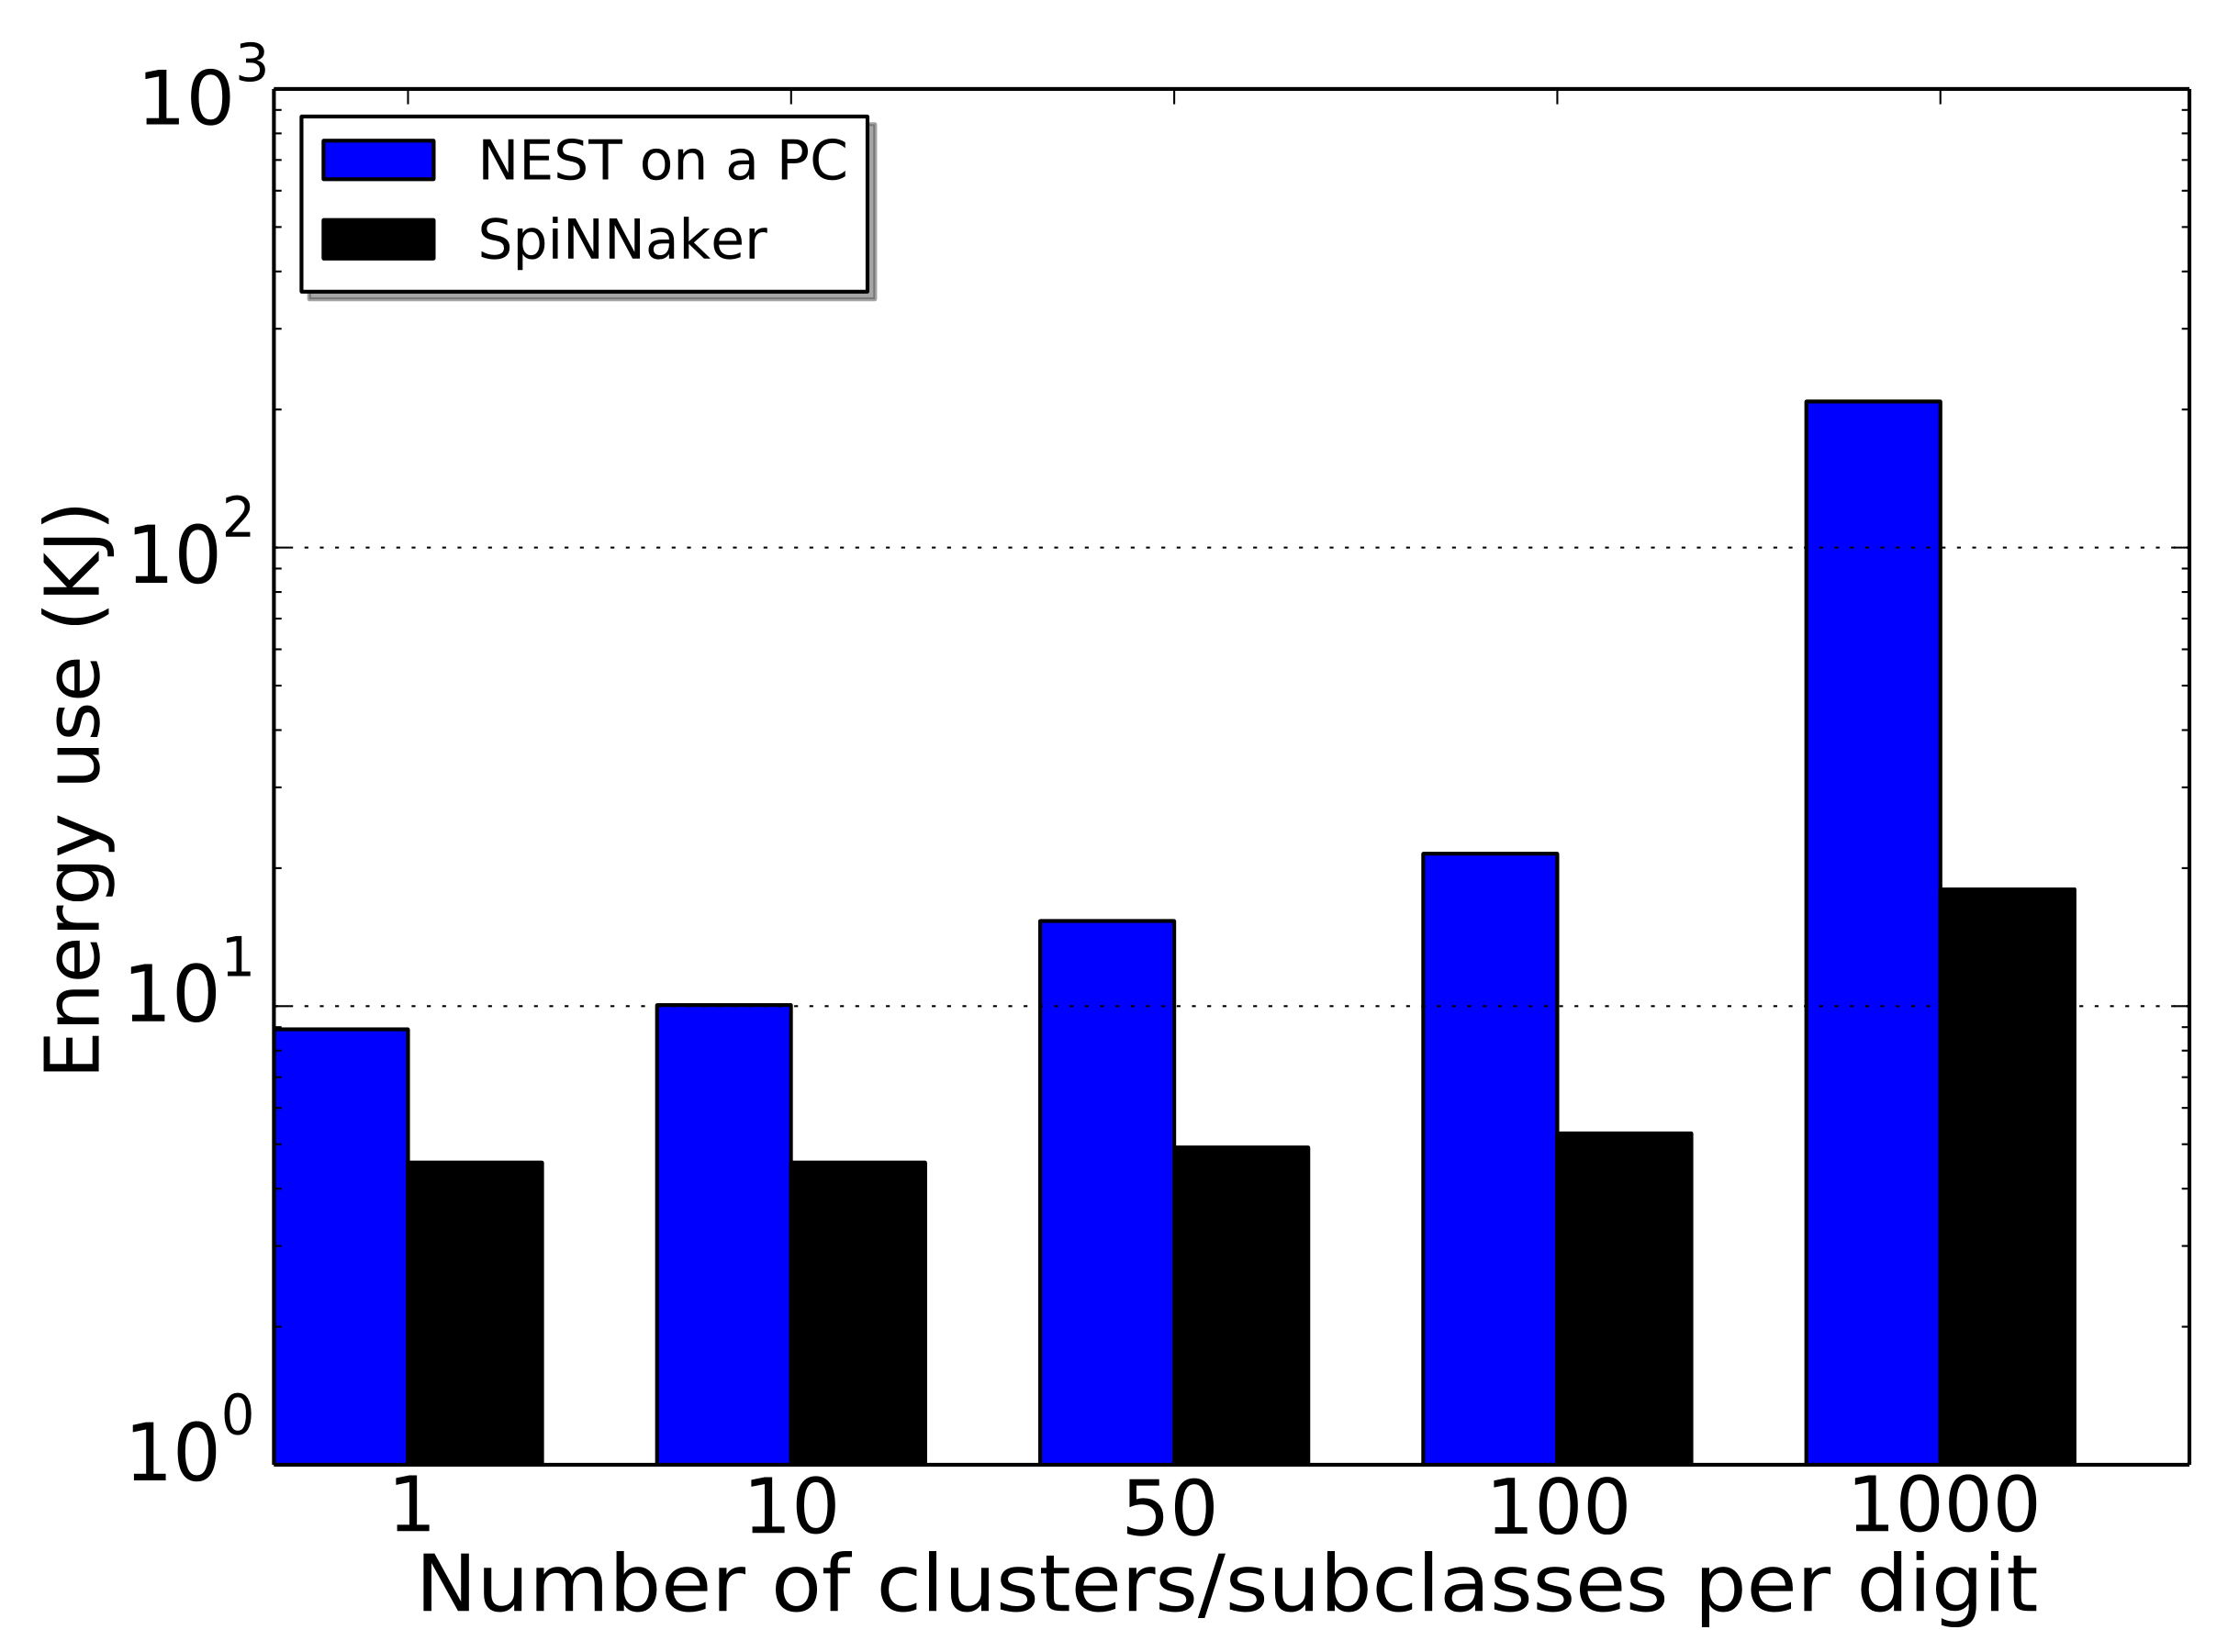
\includegraphics[width=0.6\textwidth]{pics_bench/fig8.jpg}
	\caption[Energy usages of different network size.]{Energy usages of different network size both using NEST (blue) on a PC and SpiNNaker (black).}
	\label{fig:energy}
\end{figure}
%\subsection{Case Study II}
%% brief intro about dbn
%This section aims to review and reinterpret results from previously published studies  \citep{Stromatias2015LiveDemo,Stromatias2015scalable,stromatias2015robustness}, which utilised the identical off-line trained\footnote{\url{https://github.com/dannyneil/edbn/}} spiking DBN as presented by \citep{o2013real}.
%
%Deep learning architectures and, in particular, Convolutional Networks~\citep{lecun1998gradient} and Deep Belief Networks (DBNs)~\citep{hinton2006fast} have been characterised as one of the breakthrough technologies of the decade~\citep{MIT_TechReview}. One of the advantages of these type of network is that their performance can be increased by adding more layers~\citep{hinton2006fast}.
%
%However, state-of-the-art deep networks comprise a large number of layers, neurons and connections resulting in high energy demands, communication overheads, and high response latencies. This is a problem for mobile and robotic platforms which may have limited computational and power resources but require fast system responses. 
%
%
%% about oneils model 
%\citep{o2013real} proposed a method to map off-line trained DBNs into a spiking neural network and take advantage of the real-time performance and energy efficiency of neuromorphic platforms. This led initially to an implementation on an event-driven Field-Programmable Gate Array (FPGA) called Minitaur~\citep{neil2014minitaur} and then on the SpiNNaker platform~\citep{Stromatias2015scalable}.
%%This section aims to review and reinterpret results from previously published studies  \citep{Stromatias2015LiveDemo,Stromatias2015scalable,stromatias2015robustness}, which utilised the identical off-line trained\footnote{\url{https://github.com/dannyneil/edbn/}} spiking DBN as presented by \citep{o2013real}.
%This particular DBN comprises 784 neurons for the input layer, two hidden layers with 500 neurons each, and an output layer with 10 neurons. This is abbreviated as a 784-500-500-10 architecture.
%Simulations take place on a software spiking neural network simulator, Brian~\citep{goodman2008brian}, and results are verified on the SpiNNaker platform.
%
%\subsubsection{Training}
%
%DBNs consist of stacked Restricted Boltzmann Machines (RBMs), which are fully connected recurrent networks but without any connections between neurons in the same layer. Training is performed unsupervised using the standard Contrastive Divergence (CD) rule~\citep{hinton2006fast} and only the output layer is trained in a supervised manner. The main difference between spiking DBNs and traditional DBNs is the activation function used for the neurons.~\citep{o2013real} proposed the use of the Siegert approximation~\citep{Jug_etal_2012} as the activation function, which returns the expected firing rate of an LIF neuron (Equation~\ref{eq:LIF}) given the input firing rates, the input weights, and standard neuron parameters. Further details regarding the training process can be found in \citep{o2013real}.
%
%\subsubsection{Testing}
%After the training process the learnt synaptic weights can be used in a spiking neural network which consists of LIF neurons with delta-current synapses. Table~\ref{Tab:NeuralParams} shows the LIF parameters used in the simulations.
%These parameters were chosen by~\citep{o2013real} to train this spiking DBN network. 
%%Later,~\citep{neil2014minitaur} used the identical offline trained network to map it on an event-driven FPGA implementation called Minitaur.
%Using the same network and parameters allowed us to have a direct comparison between the power requirements and numerical precision, for different software and hardware platforms (Matlab, Brian, Minitaur, SpiNNaker).
%
%\begin{table}[hbbp]
%	\centering
%	\caption{\label{Tab:NeuralParams}Default parameters of the Leaky Integrate-and-Fire Model used in the DBN simulations.}
%	\bgroup
%	\def\arraystretch{1.3}
%	\begin{tabular}{c c c}
%		%\hline
%		Parameters & Values & Units \\
%		\hline
%		tau\_m & 5 & s\\
%		%\hline
%		tau\_refrac & 2.0 & ms\\
%		%\hline
%		v\_reset & 0.0 & mV\\
%		%\hline
%		v\_rest & 0.0 & mV\\
%		%\hline
%		v\_thresh & 1.0 & mV\\
%		%\hline
%	\end{tabular}
%	\egroup
%\end{table}
%
%The pixels of each MNIST digit from the testing set are converted into Poisson spike trains as described in Section~\ref{sec:poissonian}. %with a rate proportional to the intensity of their pixel, while their firing rates are scaled so that the total firing rate of the input population is constant~\citep{o2013real}.
%The CA was chosen as the performance metric of the spiking DBN, which is the percentage of the correctly classified digits over the whole MNIST testing set.
%
%\subsubsection{Evaluation}
%Neuromorphic platforms may have limited hardware resources to store the synaptic weights~\citep{schemmel2010wafer,merolla2014million}. In order to investigate how the precision of the weights affects the CA of a spiking DBN the double-precision floating-point weights of the offline-trained network were converted to various fixed-point representations. The following notation will be used throughout this paper, Q\textit{m.f}, where \textit{m} signifies the number of bits for the integer part (including the sign bit) and \textit{f} the number of bits used for the fractional part.
%
%Figure~\ref{Fig:brianCAfiringrate} shows the effect of reduced weight bit precision on the CA for different input firing rates on the Brian simulator.
%%To validate the results of the software simulator simulations ran on SpiNNaker for a weight resolution of Q3.8.
%Using the same weight precision of Q3.8, SpiNNaker achieved a CA of 94.94\% when $1,500$~Hz was used for the input population~\citep{Stromatias2015scalable}. With the same firing rates and weight precision, Brian achieved a CA of 94.955\%. Results are summarised in Table~\ref{tab:casimulators}.
%The slightly lower CA of the SpiNNaker simulation indicates that not only the weight precision but also the precision of the membrane potential affects the overall classification performance.    
%\citep{stromatias2015robustness} showed that spiking DBNs are capable of maintaining a high CA even for weight precisions down to Q3.3, while they are also remarkably robust to high levels of input noise regardless of the weight precision. 
%\begin{figure}[hbt!]
%	\centering
%	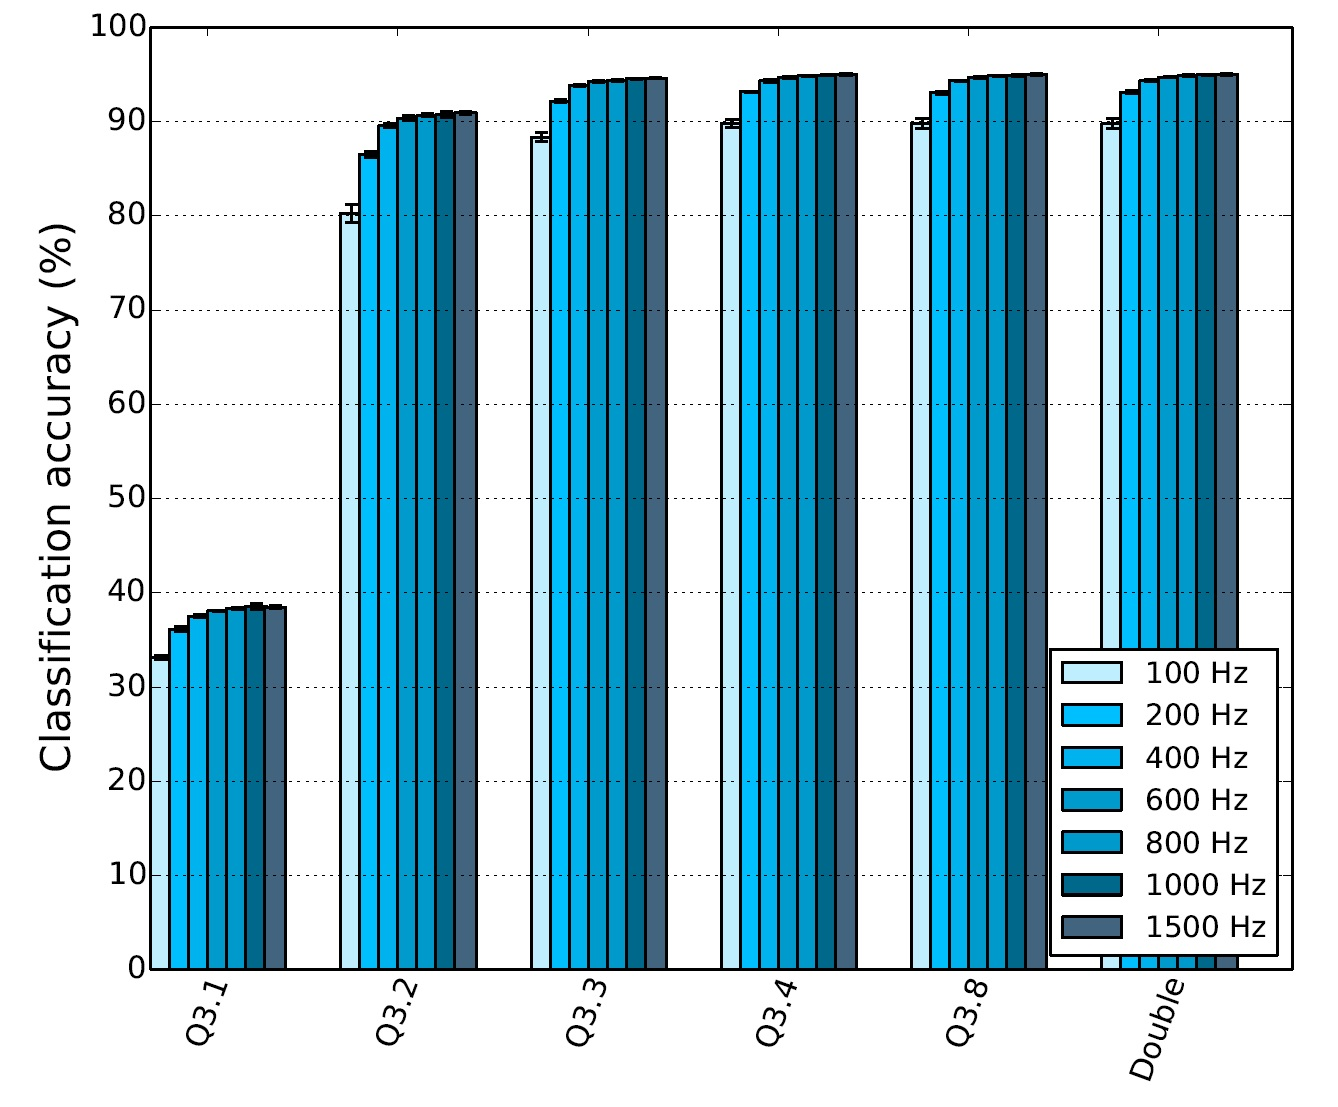
\includegraphics[width=0.6\textwidth]{pics_bench/fig9.jpg}
%	\caption{DBN classification accuracy (CA) as a function of the weight bit precision for different input firing rates \citep{stromatias2015robustness}.}
%	\label{Fig:brianCAfiringrate}
%\end{figure} 
%
%
%\begin{table}[h]
%	\caption{Classification accuracy (CA) of the same DBN running on different platforms.}
%	\begin{center}
%		\bgroup
%		\def\arraystretch{1.4}
%		\begin{tabular} {c c c}
%			Simulator & CA (\%) & Weight Precision \\
%			\hline
%			Matlab & 96.06 & Double floating point\\
%			Brian & 95.00 & Double floating point\\
%			Brian & 94.955 & Q3.8\\
%			SpiNNaker & 94.94 & Q3.8\\
%			%    \hline
%		\end{tabular}
%		\egroup
%		\label{tab:casimulators}
%	\end{center}
%\end{table}
%
%A similar experiment to the one presented for Case Study I was performed; its purpose was to establish the relation that input spike rates hold with latency and classification accuracy.
%The input rates were varied from 500~Hz to $2,000$~Hz and the results are summarised in Figure~\ref{Fig:brianLatency}. Simulations ran in Brian for all $10,000$ MNIST digits of the testing set and for 4 trials. Figure~\ref{Fig:spinnLatency1500hz} shows a histogram of the classification latencies on SpiNNaker when the input rates are $1,500$~Hz. The mean classification latency for the particular spiking DBN on SpiNNaker is 16~ms which is identical to the Brian simulation seen in Figure~\ref{Fig:brianLatency}.
%
%
%\begin{figure}[hbt!]
%	\centering
%	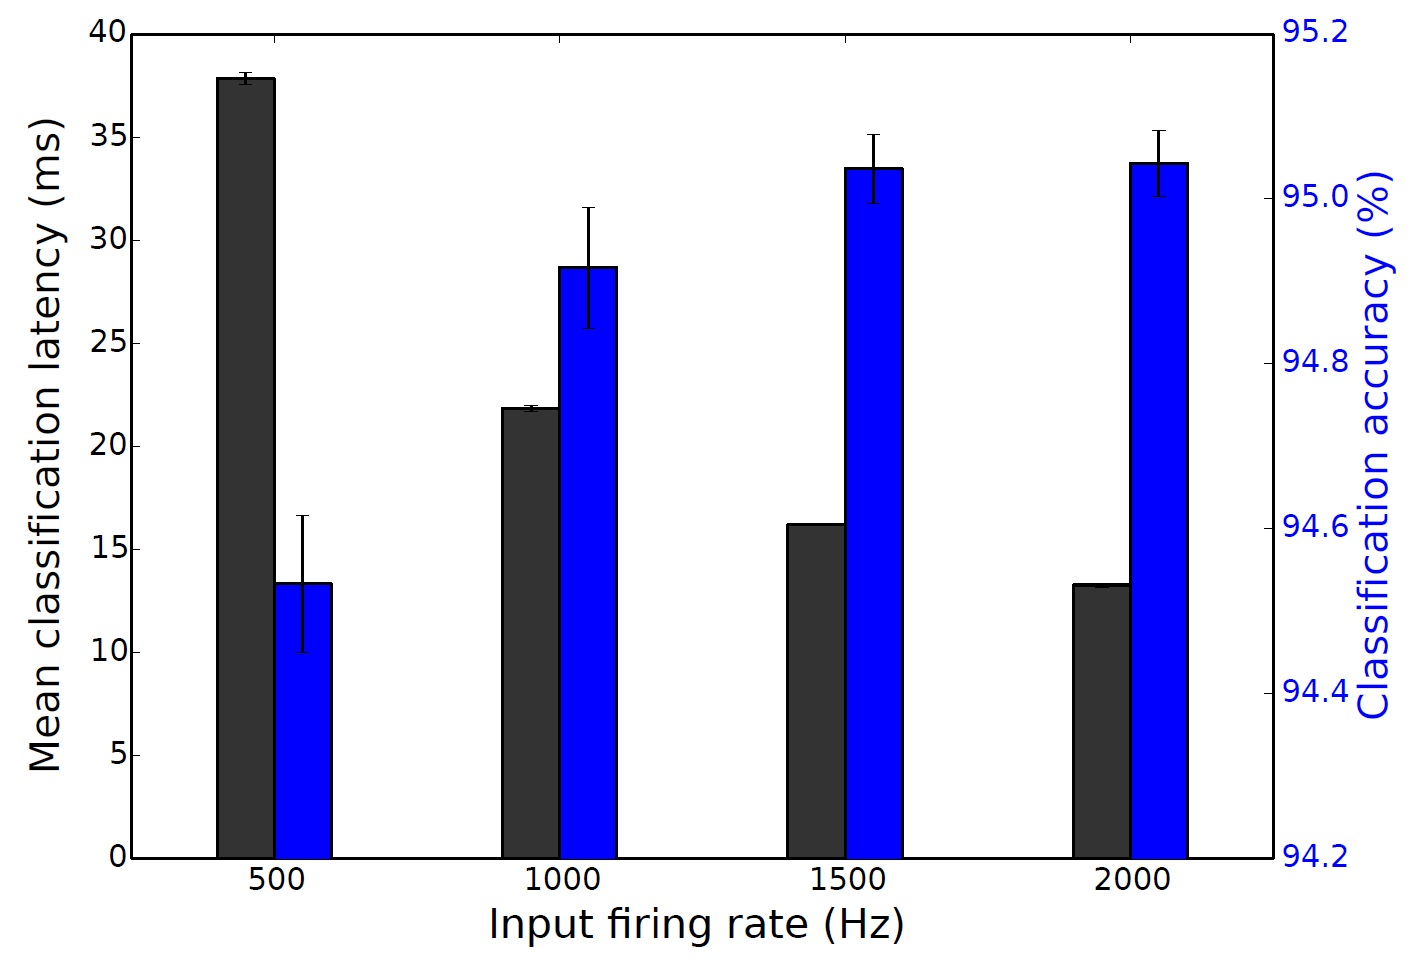
\includegraphics[width=0.6\textwidth]{pics_bench/fig10.jpg}
%	\caption{Mean classification latency (black) and classification accuracy (blue) as a function of the input firing rate for the spiking DBN. Results are averaged over 4 trials, error bars show standard deviations \citep{Stromatias2015scalable}.}
%	\label{Fig:brianLatency}
%\end{figure} 
%
%
%
%\begin{figure}[hbt!]
%	\centering
%	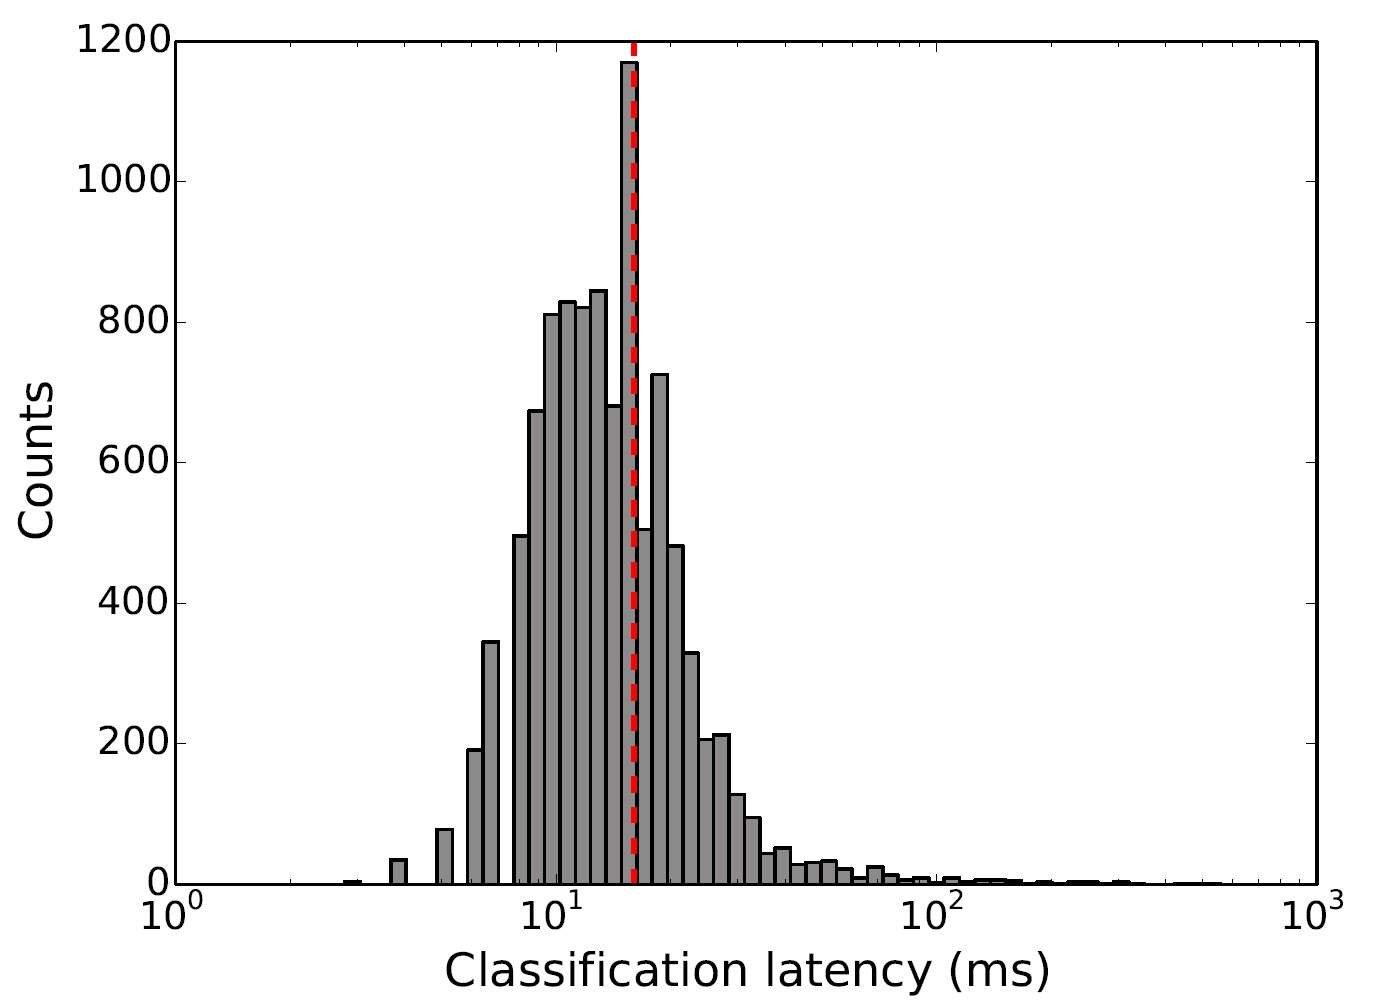
\includegraphics[width=0.6\textwidth]{pics_bench/fig11.jpg}
%	\caption{Histogram of the classification latencies for the MNIST digits of the testing set when the input rates are set to $1,500$~Hz. The mean classification latency of the spiking DBN on SpiNNaker is 16 ms \citep{Stromatias2015scalable}.}
%	\label{Fig:spinnLatency1500hz}
%\end{figure} 
%
%Finally, this particular spiking DBN ran on a single SpiNNaker chip (16 ARM9 cores) and dissipated about 0.3~W when $1,500$ spikes per second per digit were used.
%The number of generated synaptic events was $1.88$M~Sopbs and less than 2.97~KJ of energy was consumed running the whole testing set over $10,000$~s, as seen in Figure~\ref{Fig:spinnchipPower}. The identical network executed on Minitaur~\citep{neil2014minitaur}, an event-driven FPGA implementation, dissipated 1.5~W when $1,000$ spikes per image were used, and achieved a CA of 92.0\%.
%
%\begin{figure}[hbt!]
%	\centering
%	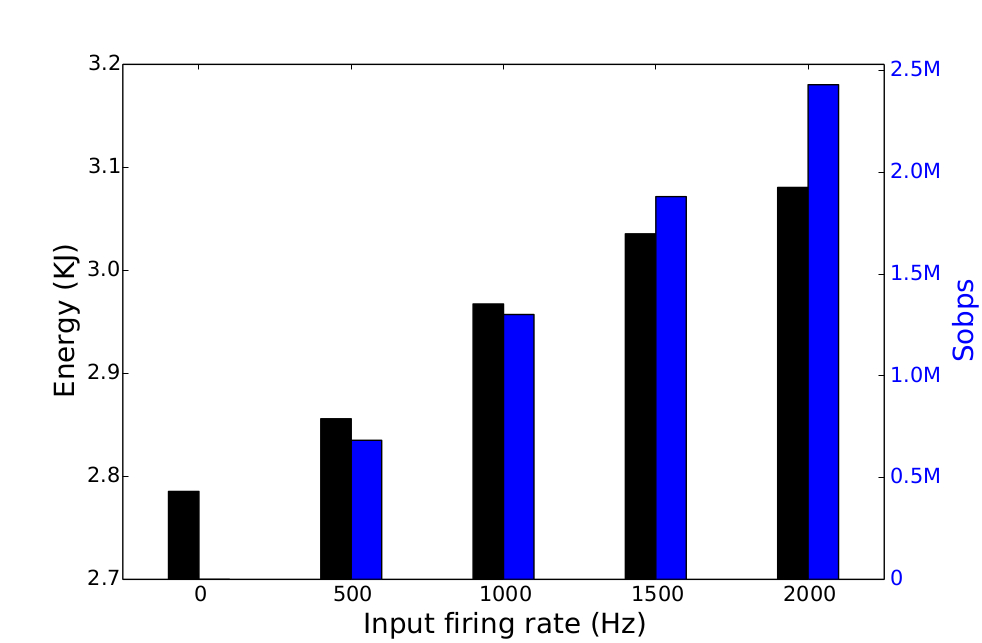
\includegraphics[width=0.6\textwidth]{pics_bench/fig12_m.jpg}
%	\caption{
%		Total energy consumption (black) and number of SE per second (blue) of a spiking DBN running on a single SpiNNaker chip as a function of the total input firing rate.}
%	\label{Fig:spinnchipPower}
%\end{figure} 

\section{Summary}
\label{sec:summ}
This chapter put forward the NE dataset as a unified resource to measure progress quantitatively within the field of neuromorphic vision.
The NE dataset and the complementary evaluation methodology make it possible to (1) provide objective comparisons of vision based SNN models and their implementation on neuromorphic platforms;
(2) compare of SNNs with conventional recognition methods by using converted spike representations of the same vision databases;
(3) measure the state-of-the-art performance in spike-based visual recognition;
and (4) promote future research into rapid and low energy recognition.
%As far as we know, this is the first attempt at benchmarking neuromorphic vision recognition by providing public a spike-based dataset and evaluation metrics.
In accordance with the suggestions from~\cite{tan2015bench}, the evaluation metrics highlight the strengths of spike-based vision tasks: low latency and energy efficiency.
% and the dataset design also promotes the research into rapid and low energy recognition (e.g. flashing digits).

A benchmark system is evaluated using the Poissonian subset of the NE15-MNIST dataset.
%The models were described and their performance on accuracy, network latency, simulation time and energy usage were presented.
This example benchmarking system demonstrates a recommended way of using the dataset, describing the SNN models and evaluating the system performance.
%They provide a baseline for comparisons and encourage improved algorithms and models to make use of the dataset.
The case study provides a baseline for robust comparisons of other SNN models and their hardware implementations.


%It contains spike-based versions of existing widely-used databases in the vision recognition field.
%Since new problems will continue to arise before vision becomes a solved question, the dataset will evolve as research progresses. 
%The conversion methods for transforming images and videos into spike trains will advance. The number of vision datasets will increase and the corresponding evaluation methodologies will evolve.
%The dataset aims to provide unified spike-based vision benchmarks and complementary evaluation methodologies to assess the performance of SNN algorithms.

